\chapter{The Drill Operator}
\label{chapter:DrillOperator} 

As discussed in Section \ref{section:SurfaceRepresentations}, common representations of terrain data have several shortcomings that limit their utility and accuracy in many applications. Simply storing spatial terrain data, with no regard for the physical process of the generation of the terrain, perpetuates these shortcomings by limiting how closely these representations can mimic real-world terrain and the formations found within. The physics of terrain formation should not be an afterthought when encoding a surface, but instead the focus of the representation.

With this in mind, this chapter presents the \emph{drill operator}, a mathematical operation that carves out terrain by ``drilling'' down into it along the segments (individual branches of the tree structure) of its extracted channel network, changing its shape to fit the channel's profile at each position along the channel's length. 
This work is directly influenced by the work of Franklin et al. \cite{wrf-autocarto-2006}, in which the authors introduce the idea of ``scooping'' the terrain. This idea of representing the terrain with a series of mathematical operations was the main influence of the drill operator.
% Also provided is the results of a series of accuracy tests on a real terrain dataset, providing evidence of the utility of the drill operator.

\section{The Terrain's Hydrography}
\label{section:ChannelNetworkExtraction}

\begin{figure}[t]
\begin{center}
  \begin{minipage}{0.49\linewidth} 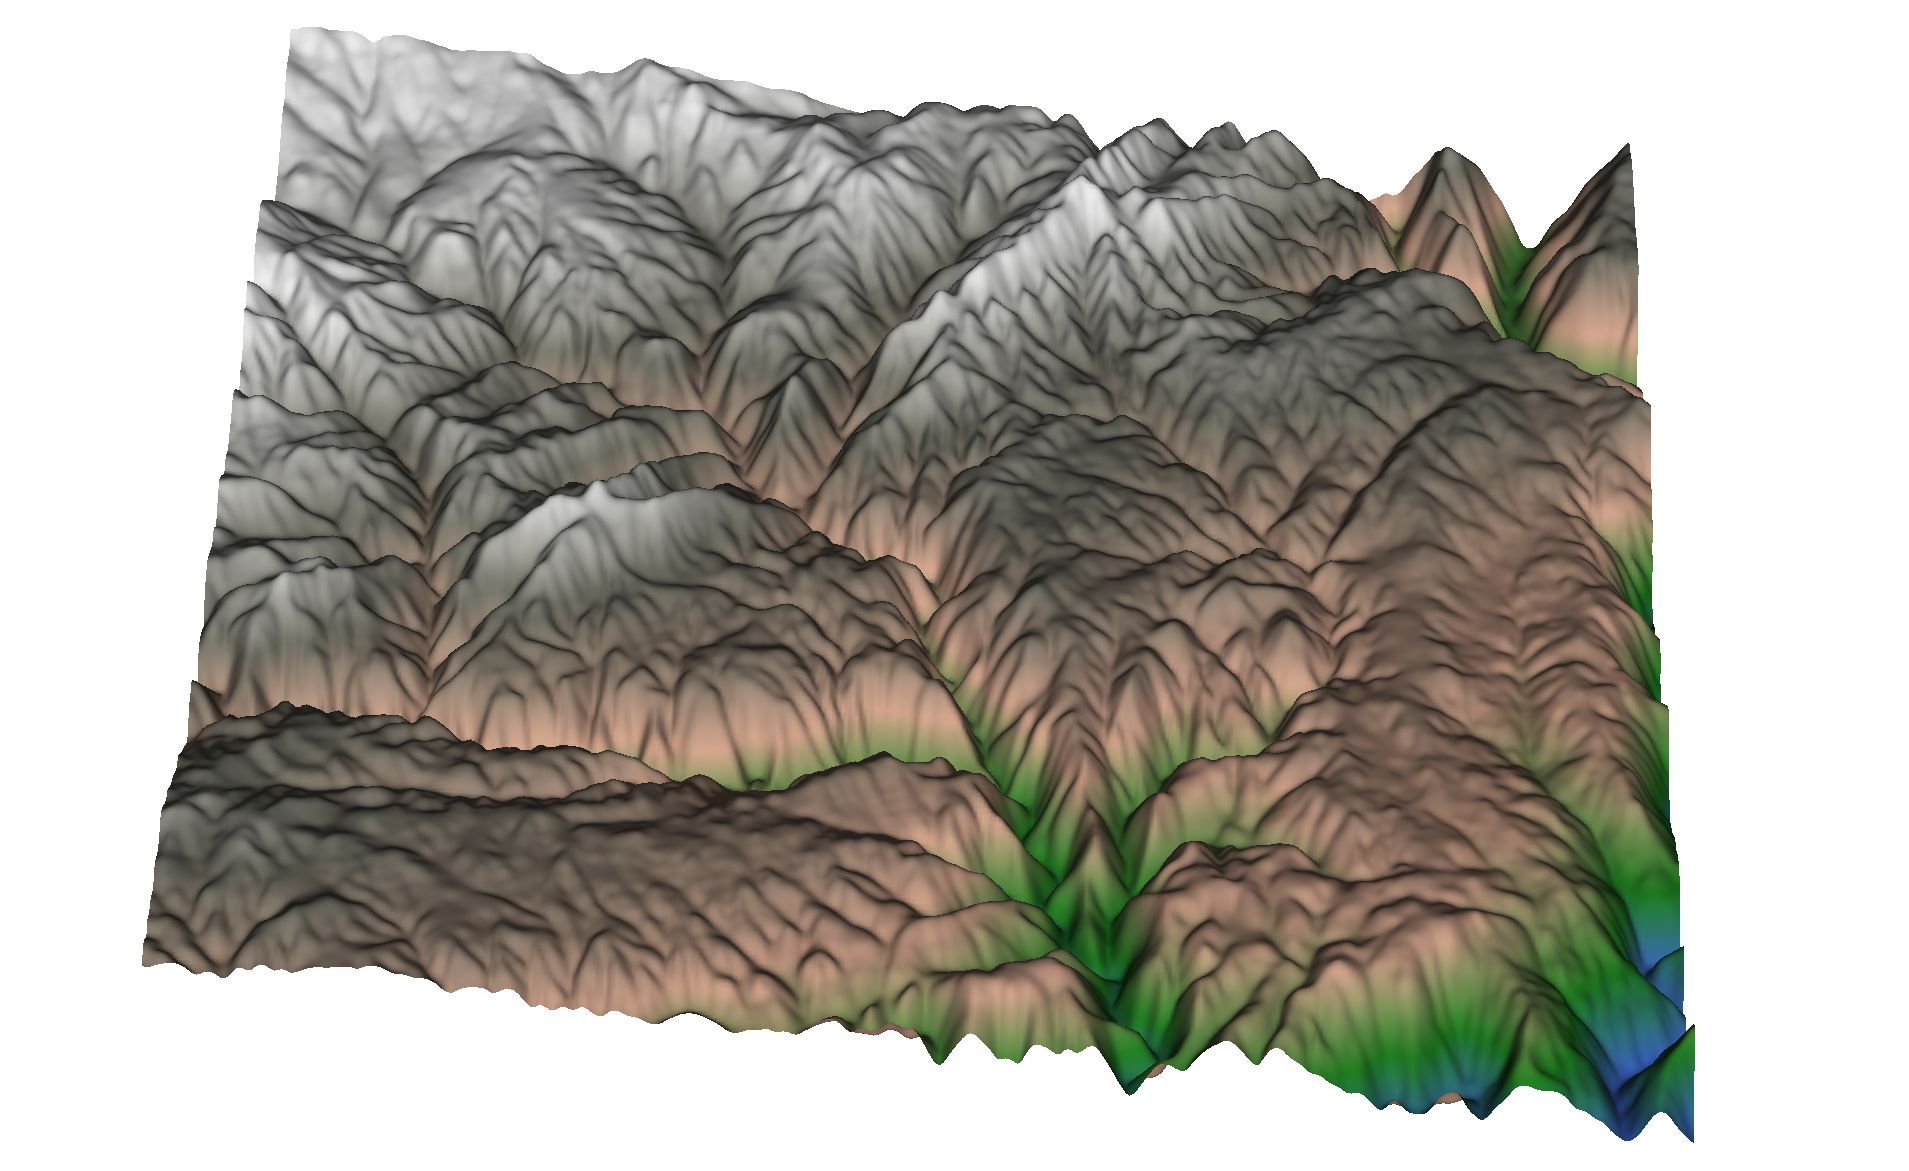
\includegraphics[width=0.99\linewidth]{images/mtn2_original.jpg} \\ \centering Original dataset \end{minipage}
  \begin{minipage}{0.49\linewidth} 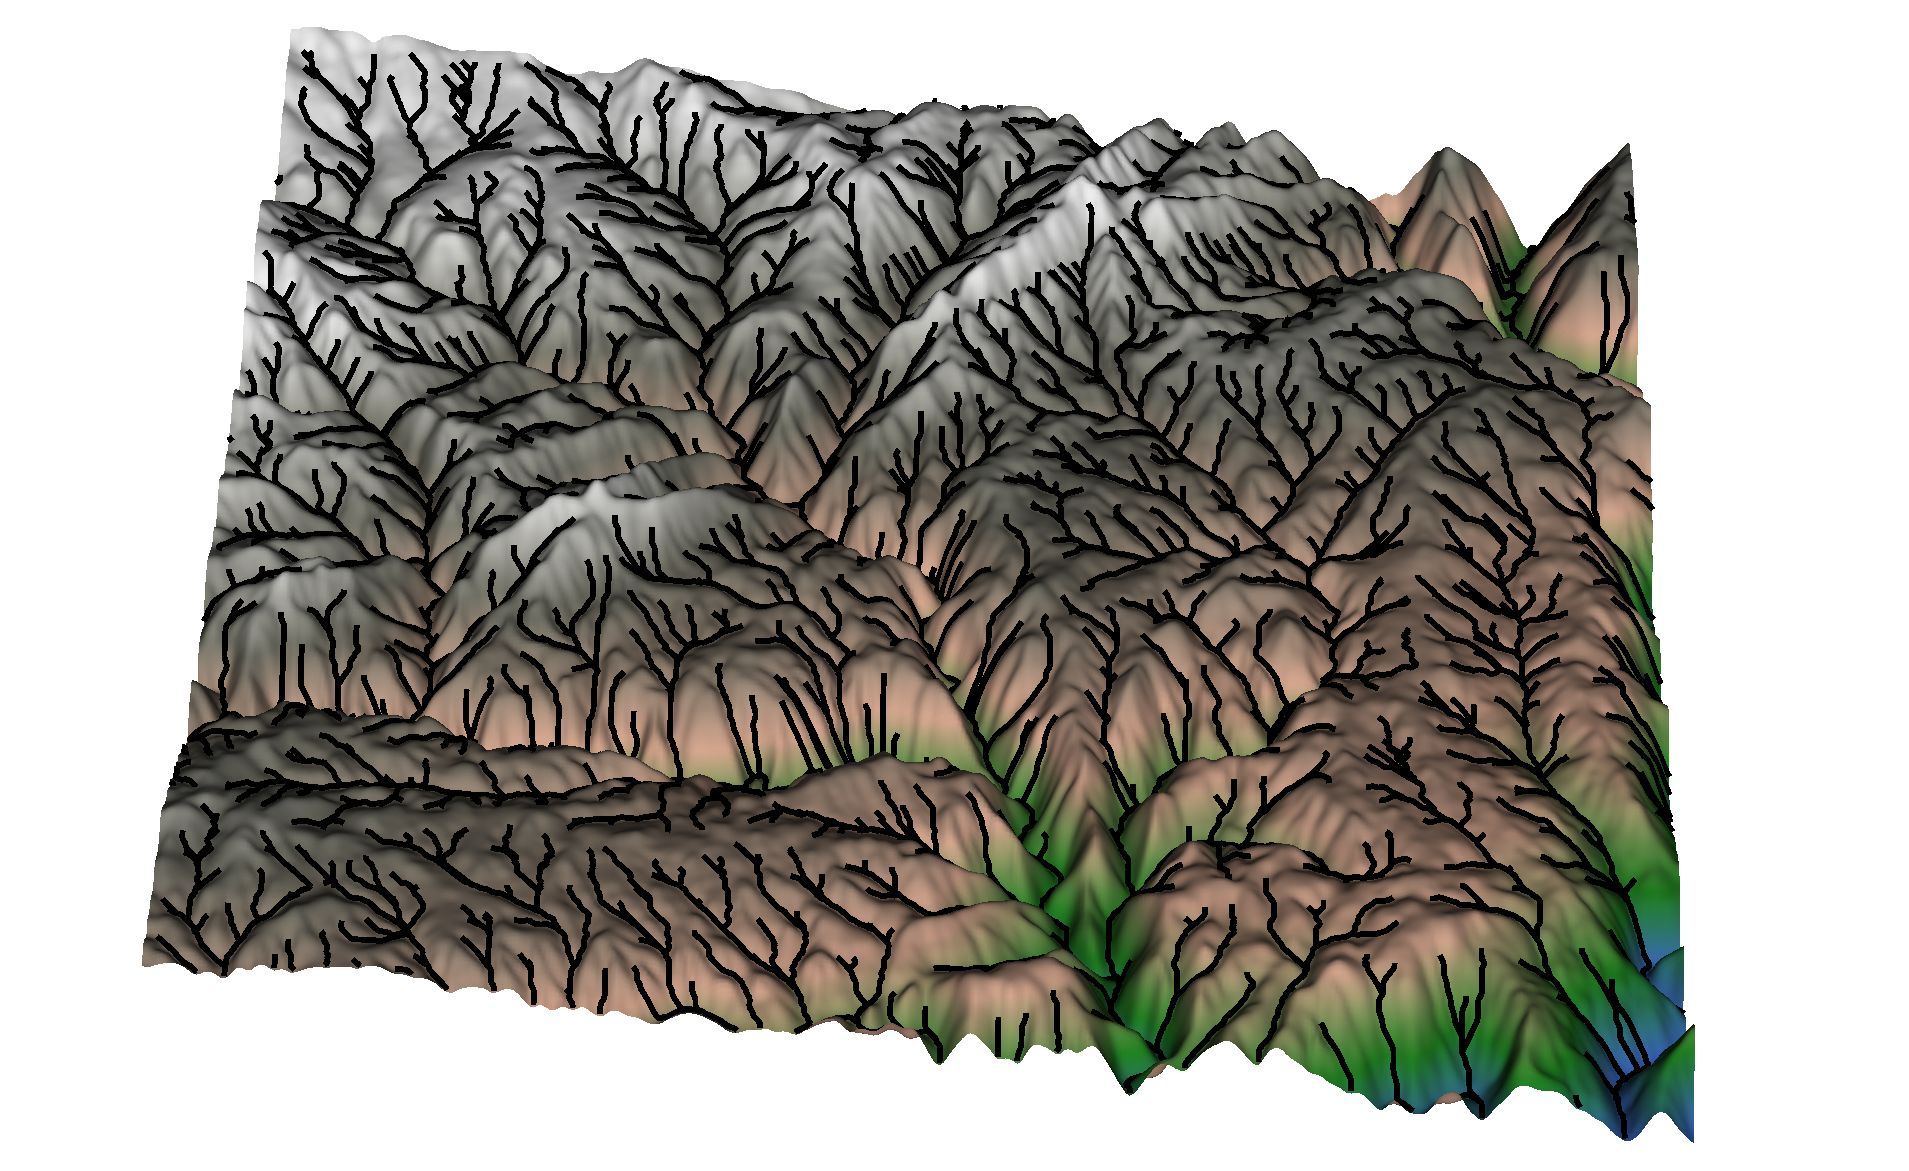
\includegraphics[width=0.99\linewidth]{images/mtn2_T25.jpg} \\ \centering $\tau = 25$ \end{minipage} \\
  \begin{minipage}{0.49\linewidth} 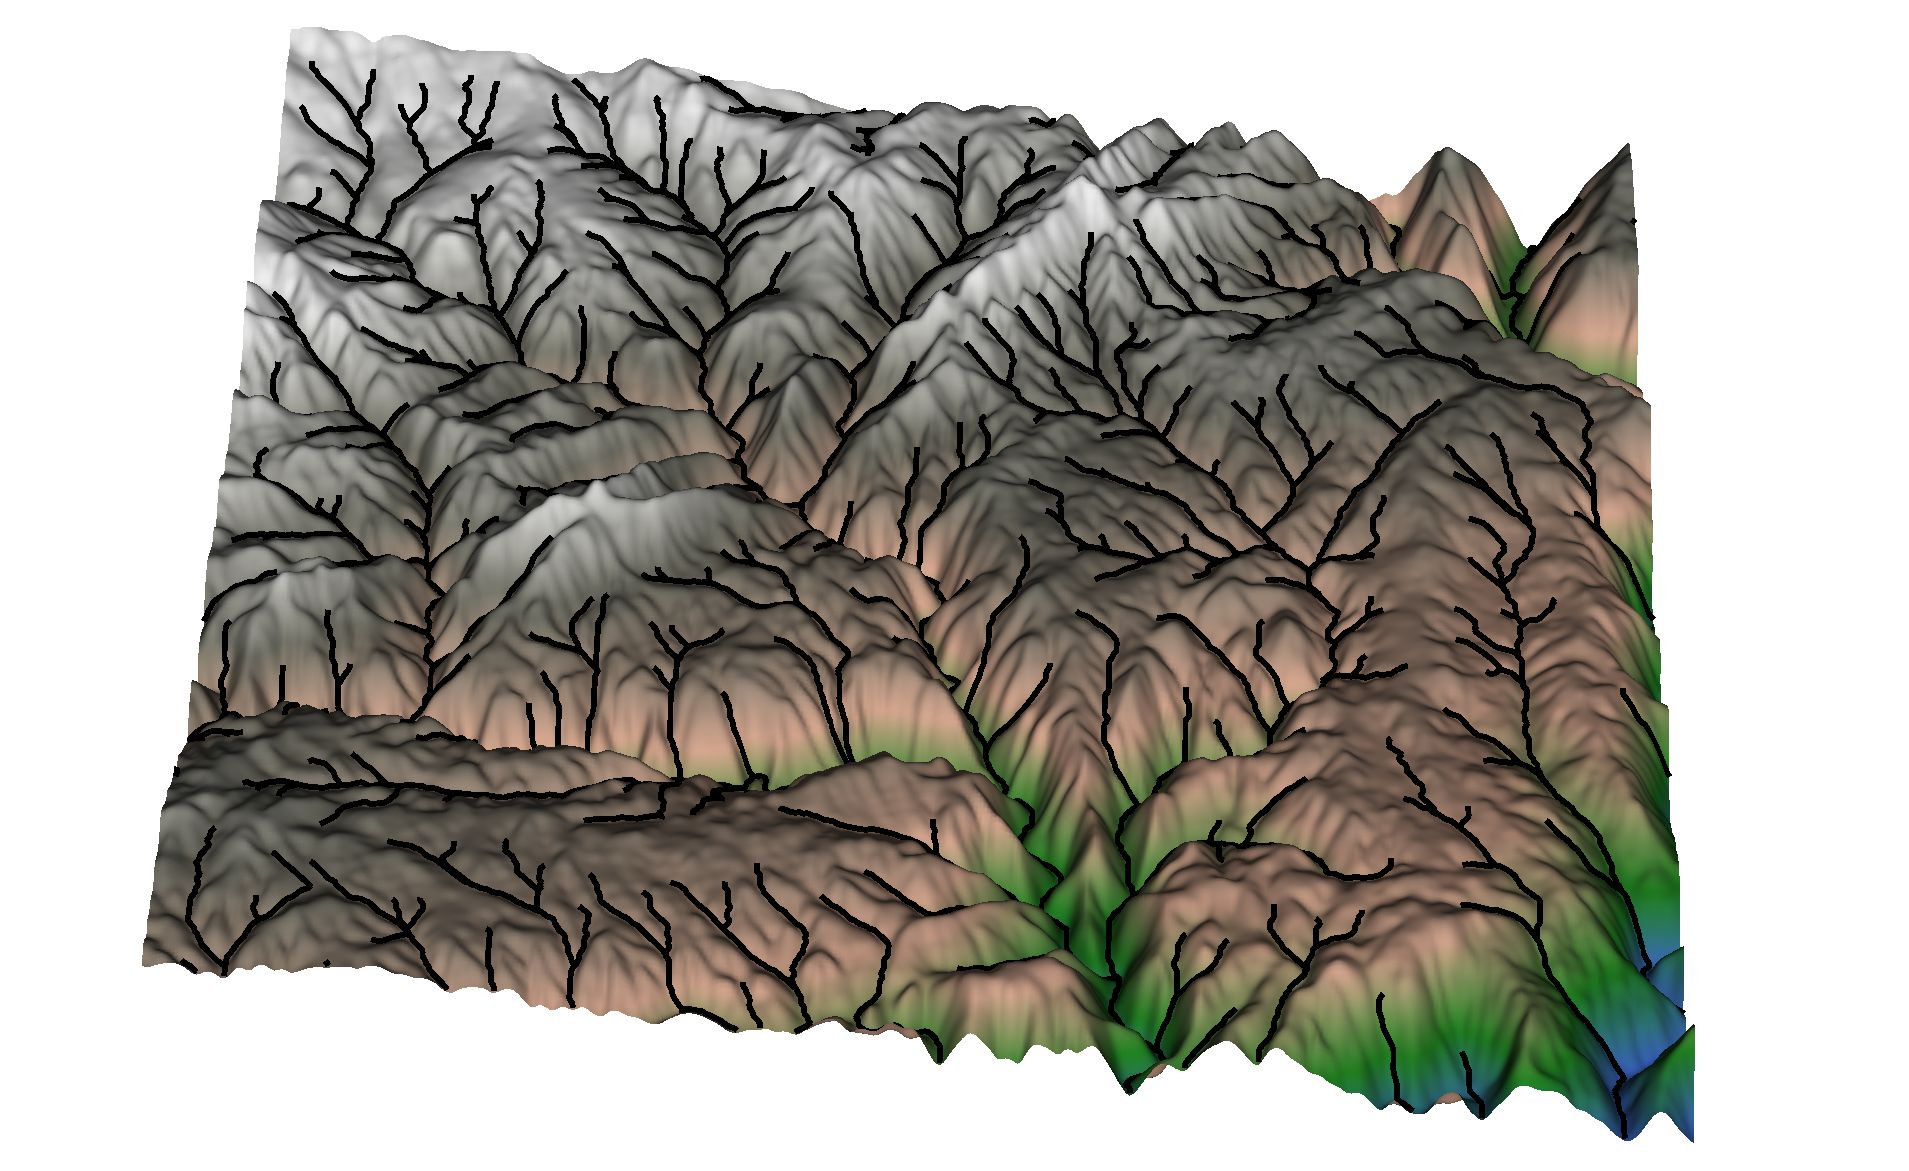
\includegraphics[width=0.99\linewidth]{images/mtn2_T100.jpg}\\ \centering $\tau = 100$ \end{minipage}
  \begin{minipage}{0.49\linewidth} 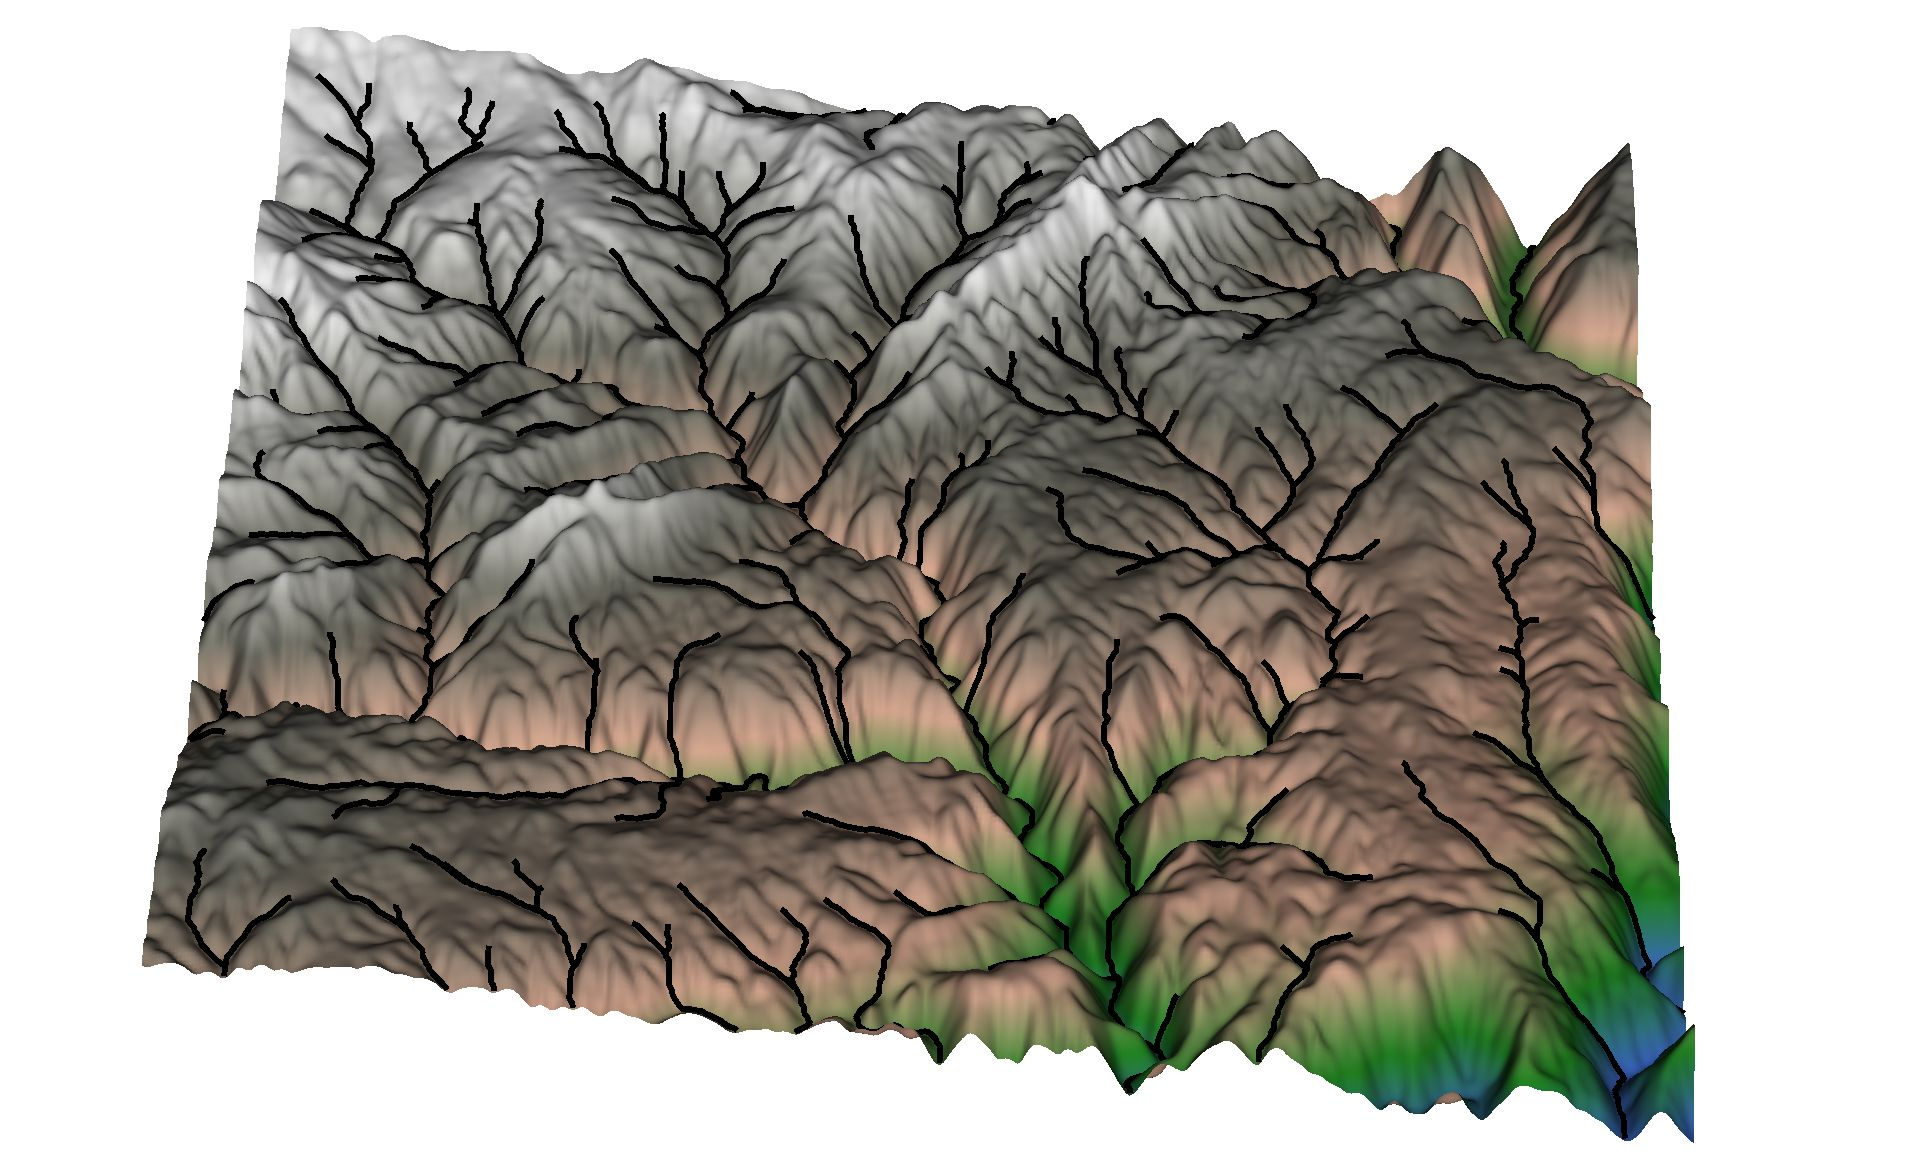
\includegraphics[width=0.99\linewidth]{images/mtn2_T200.jpg}\\ \centering $\tau = 200$ \end{minipage}
\end{center}
\caption[Four mountain datasets with extracted channel networks]{\label{figure:mtn2_original} Four depictions of a $400 \times 400$ mountainous dataset (MTN2 from Figure \ref{figure:SixDatasets}) visualized as a height field of pixels. Color indicates elevation, where white is the highest elevation, followed by brown, then green, and finally blue, which indicates the lowest elevation. Below each data set is the threshold value used to extract the channel network depicted on the surface of each terrain. Notice the difference in the densities of the channel pixels as the threshold increases.}
\end{figure}

For this and many other applications presented in this thesis, it is necessary to determine which pixels of the terrain are deemed to be ``important''. That is, which pixels are part of the terrain formations that are of consequence when terrain is represented, compressed, and analyzed. These pixels are those in the terrain's channel network, and popular methods for their extraction were discussed in Section \ref{section:PriorLiteratureChannelNetworkExtraction}. Most channel network extraction methods determine the flow direction matrix, and then use the flow accumulation algorithm presented by O'Callaghan and Mark \cite{OCALLAGHAN-Extraction} to extract the pixels of the channel network. In this work, the threshold $\tau$ applied to the flow accumulation matrix determined by this method can also be based on a user defined percentage value $r$, which represents a percentage of pixels of the terrain to be included in the channel network.
An example of the effect various values of $\tau$ can have on the channel network can be seen in Figure \ref{figure:mtn2_original}.
The method used for determining flow direction in this thesis was presented by Metz et al. \cite{hess-15-667-2011} in 2011, and is the algorithm currently used in the \textit{GRASS} software.

\subsection{Extracting the Channel Network}

Given a height field $T$ made up of $n$ pixels $\textbf{p}_i$ with elevation values, the algorithm uses a bottom-up elevation-based priority approach to determine flow direction. It uses a priority queue $Q$ which holds pixels prioritized by elevation first and order-of-input into the queue second. 

First, the set of possible flow outlet points are determined. These points are generally the pixels along the border (as in this work), but can also be any sinks identified within the terrain. These pixels are added to $Q$. Then each pixel of highest priority (lowest elevation) is processed in order until $Q$ is empty. For each pixel $\textbf{p}_i$, all neighbors of $\textbf{p}_i$ that have not yet been processed (placed in $Q$) have their flow directions set toward $\textbf{p}_i$, and are added to $Q$. After each $\textbf{p}_i$ has been processed in this manner (meaning $Q$ is empty), the flow direction matrix will be generated.

% In order to extract the channel network once the flow direction matrix is calculated, a threshold $\tau$ is applied to the pixels 

This method has several advantages over that presented by O'Callaghan and Mark. First, there is no need to pre-process the terrain to take care of pits and basins. 
Normally, without complex additional rules added to the algorithm, pits halt flow direction calculation because no neighbor has a lower elevation. 
Basins cause problems because they are created by many neighboring pixels with the same elevation values, so tie-breaking processes are necessary and add a level of complexity to the algorithm.
Since this method ignores neighbor heights and only takes advantage of the fact that the neighboring pixels are adjacent to the current, pits and basins are no longer an issue. Each pixel simply flows in the direction of the outlet it is ``closest'' to, elevation-wise. 
% While this is not always the case, no method yet presented in the area produces a flow network guaranteed to be correct all of the time, nor is such a request feasible.

Secondly, the method is fast ($O\left(n \log{n}\right)$), which is based on the speed of the priority queue implementation, and so advances in priority queue implementation lead directly to speedups for this algorithm. Thirdly, the algorithm provides a pixel list ordered from lowest elevation to highest, which is saved and used in several other portions of this work, saving a great deal of time in the future. The fact that pixels are processed in a bottom-up order allows for future algorithms to be optimized for this ordering. 

\subsection{Choosing a Flow Threshold}
\label{section:ChoosingAFlowThreshold}

% As described in Section \ref{section:ChannelNetworkExtraction}, to extract the channel network $N_{\tau}$ from a terrain $T$, a threshold $\tau$ is applied to $T$'s flow accumulation matrix $flowAccum_{T}$. 
% This section describes a method of determining an optimal threshold to apply to a pair of terrains to minimize the distance between their channel networks. 

\begin{figure*}[t]
\centering
\begin{minipage}[b]{0.45\linewidth}
\begin{center}
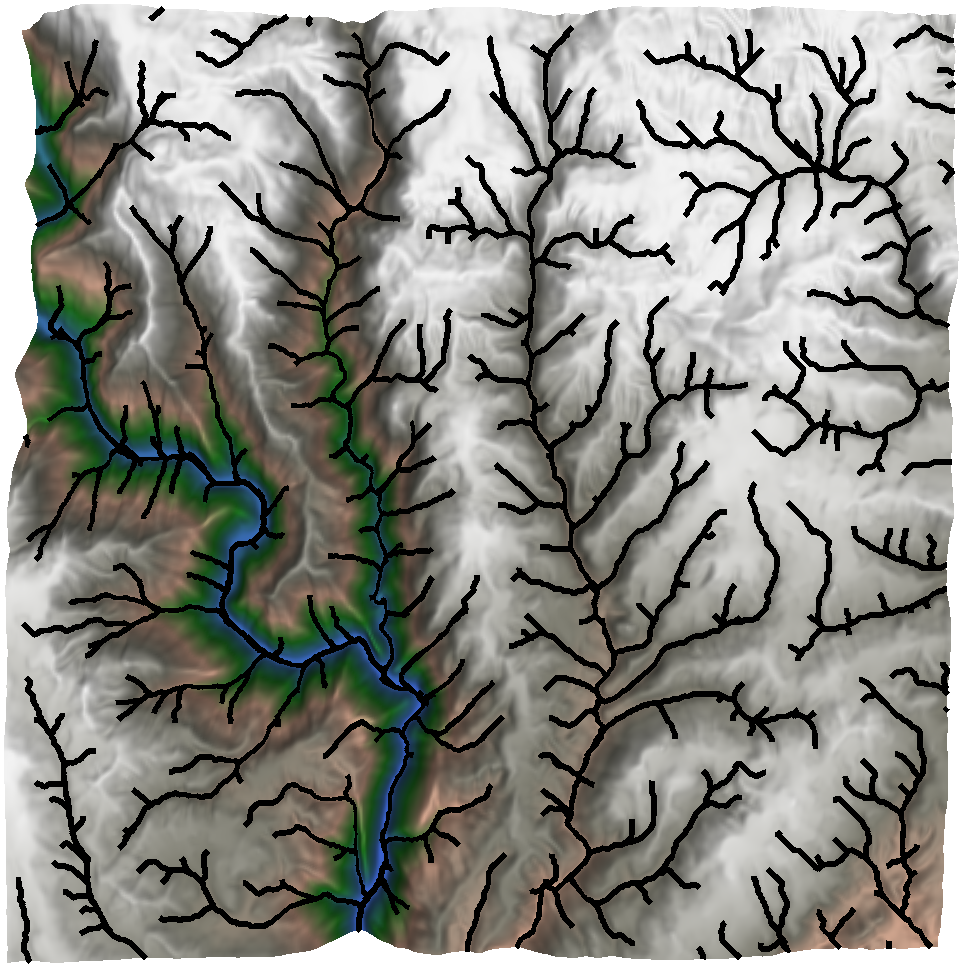
\includegraphics[width=\linewidth]{images/ChannelNetworkWithoutWeights_160_mtn3.png}
\end{center}
\end{minipage}
\begin{minipage}[b]{0.45\linewidth}
\begin{center}
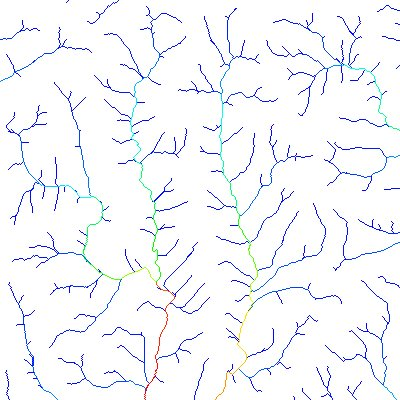
\includegraphics[width=\linewidth]{images/FlowField_mtn3_WithoutWeight.jpg}
\end{center}
\end{minipage}
\caption[An extracted channel network on MTN3 with a global threshold.]{\label{figure:ChannelNetwork_GlobalThreshold} An extracted channel network on MTN3 using one global flow threshold of 160 units of flow. Left: A bird's-eye view of the extracted channel network, with the pixels whose flow values exceed 160 units of flow shown in black. Right: A visualization of the flow accumulation matrix (after thresholding). Red indicates maximum flow, and blue indicates minimum flow. }
\end{figure*}



Traditionally, a single global threshold $\tau$ is applied to $flowAccum_{T}$,
% the flow accumulation matrix, 
and any pixels whose flow value exceeds the threshold are considered to be part of the channel network $N_{\tau}$. An example of an extracted channel network on MTN3 can be seen in figure \ref{figure:ChannelNetwork_GlobalThreshold}, in which channels are drawn in black on the terrain. The goal of any channel network extraction algorithm is to closely match the ``blue-line'' standard, or the accepted channels that a hydrologist studying the terrain in question would identify. In many cases, a single global threshold does an acceptable job identifying the intuitive placement of channels. However, one major drawback to using a single threshold is that the procedure is biased towards lower elevations, as flow accumulates in a top down fashion. Because there is less water available at the higher elevations, this creates a bias.

There have been several attempts to rectify this, such as use of other criterion for thresholding. Tarboton et al. \cite{Tarboton-OnExtraction} suggest using drainage density, constant drop procedures, or slope scaling procedures to properly weight pixels when deciding which should be included in the channel network. In this thesis, a weighting scheme is applied that assigns a different weight to the threshold for each pixel. The weight ($w_{thresh}$) is calculated as follows:

\begin{align}
  heightP & = \frac{ \textbf{p}_{z} - min\left(T\right) }{ max\left(T\right) - min\left(T\right) } \\
  indexP & = \frac{ \textbf{p}_{index} }{ |T| - 1 } \\
  w_{thresh}( \textbf{p} ) & = w_{e} * \left( heightP \right) + w_{o} * \left( indexP \right)
\label{equation:ThresholdWeightingScheme}
\end{align}


\noindent where $w_{e}$ and $w_{o}$ are linear weighting factors (such that $w_{e} + w_{o} = 1.0$). The constant values $min\left(T\right)$ and $max\left(T\right)$ are the minimum and maximum elevation found on the terrain, respectively. The pixel $\textbf{p}$ has an elevation $\textbf{p}_{z}$ and an index into the array of ordered elevations $\textbf{p}_{index}$. The term $heightP$ refers to $\textbf{p}$'s normalized position in the range of elevations, and $indexP$ to its normalized index into the array of ordered elevations. The weighting factors $w_{e}$ and $w_{i}$ allow for one or the other factor to be taken into more consideration. Equation \ref{equation:ThresholdWeightingScheme} provides a weight to be applied when considering whether pixel $\textbf{p}$ is in the channel network that takes into consideration its elevation with regard to both the maximum and minimum elevation on the terrain as well as its ranking among the rest of the pixels. This weight is applied in Algorithm \ref{algorithm:ThresholdFlow}. In practice, values of $w_{e} = 0.75$ and $w_{o} = 0.25$ work well to remove bias from the thresholding.

Another possible weighting scheme will be discussed in detail in Section \ref{section:PixelLoad}.
Using a weighted threshold allows for channels to stretch into higher elevations while minimally disrupting the lower elevations. An example of this can be seen in Figure \ref{figure:WithAndWithoutThresholdWeights}. Notice that there are more tributaries that stretch higher along the mountain peaks, filling in white areas.

% \fbox{Point them out somehow}

\begin{algorithm}[t]
\begin{algorithmic}
%   \STATE \COMMENT{For each pixel, if its flow is below the weighted threshold, set to 0}
  \FOR{$\textbf{p} = 0 \to |T|$} 
    \IF{$FlowAccum( \textbf{p} ) * w_{thresh} < \tau$}
      \STATE $FlowAccum( \textbf{p} ) \gets 0$
    \ENDIF
  \ENDFOR
\end{algorithmic}
\caption[The algorithm for applying a threshold to the $flowAccum$ matrix.]{\label{algorithm:ThresholdFlow}The algorithm for applying a threshold to the $flowAccum$ matrix.}
\end{algorithm}

\begin{figure*}[t]
\centering
\begin{tabular}{c|c}
\begin{minipage}[b]{0.45\linewidth}
\begin{center}
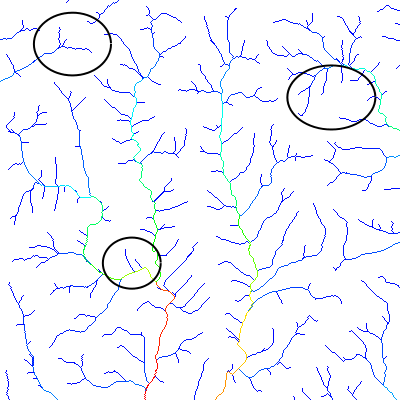
\includegraphics[width=\linewidth]{images/2DWithoutThresholdWeighting_mtn3_annotated.png}
\end{center}
\end{minipage}
&
\begin{minipage}[b]{0.45\linewidth}
\begin{center}
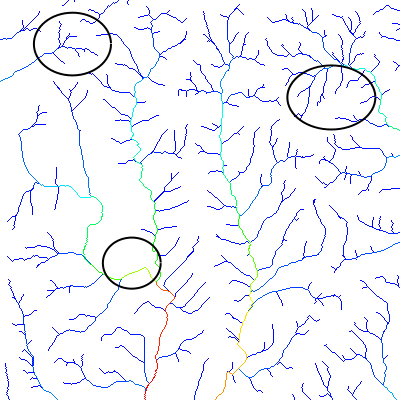
\includegraphics[width=\linewidth]{images/2DWithThresholdWeighting_mtn3_annotated.png}
\end{center}
\end{minipage} 
\end{tabular}
\caption[Two channel networks on MTN3, one without weighting and the other with.]{\label{figure:WithAndWithoutThresholdWeights} Two channel networks on the MTN3 dataset. The network to the left is extracted without using threshold weighting, while the network to the right does use it. Notice that as weighting is added, channels in higher elevations stretch for longer while channels along lower and flatter portions of the terrain disappear or become shorter. }
\end{figure*}


\begin{algorithm}[t]
\begin{algorithmic}
  \FOR{$\textbf{p} = 0 \to |T|$}
    \IF{$FlowAccum( \textbf{p} ) > 0$}
      \STATE $\textbf{p}' = lowestNeighbor( \textbf{p} )$
      \STATE $FlowAccum( \textbf{p}' ) \gets originalFlow( \textbf{p}' )$
    \ENDIF
  \ENDFOR 
\end{algorithmic}
\caption[Algorithm to fill in the gaps left by the flow threshold weighting scheme]{\label{algorithm:ChannelGapFilling}The algorithm to fill in the gaps left by the flow threshold weighting scheme.}
\end{algorithm}

Because the weighting scheme is applied to a single pixel at a time, ignoring neighbor information, it is possible that gaps appear in the channel network. Because we can assume that water flow is continuous (as discussed above), these gaps can be repaired easily. The method used is described in Algorithm \ref{algorithm:ChannelGapFilling}. Every pixel along a flow path between a source and its sink is considered part of the network.
% 
Algorithm \ref{algorithm:ChannelGapFilling} can either be applied to pixels in elevation order, or iteratively until no new pixels are discovered. 
% What we have left is a matrix of pixels belonging to the channel network. Once this matrix of channel network pixels is populated, further analysis of the network becomes possible.

Once the pixels of the channel network have been identified, the drill representation of the terrain can be determined.

\section{The Drill Representation}

For any given pixel on the terrain, $\textbf{p}_{i} \in T$, a drill shape is determined by fitting a curve to the channel profile at $\textbf{p}_{i}$, which then represents the shape of the widest drill that can conservatively fit in the channel.
The overall channel profile is represented by the union of all collected cross sections at $\textbf{p}_{i}$.
%  This process is depicted in Figure TBD. 

% \fbox{NEW IMAGE FOR NEW METHOD}

\subsection{Determining Drill Shape}

\begin{figure}[t]
\begin{center}
  \begin{minipage}{0.49\linewidth} 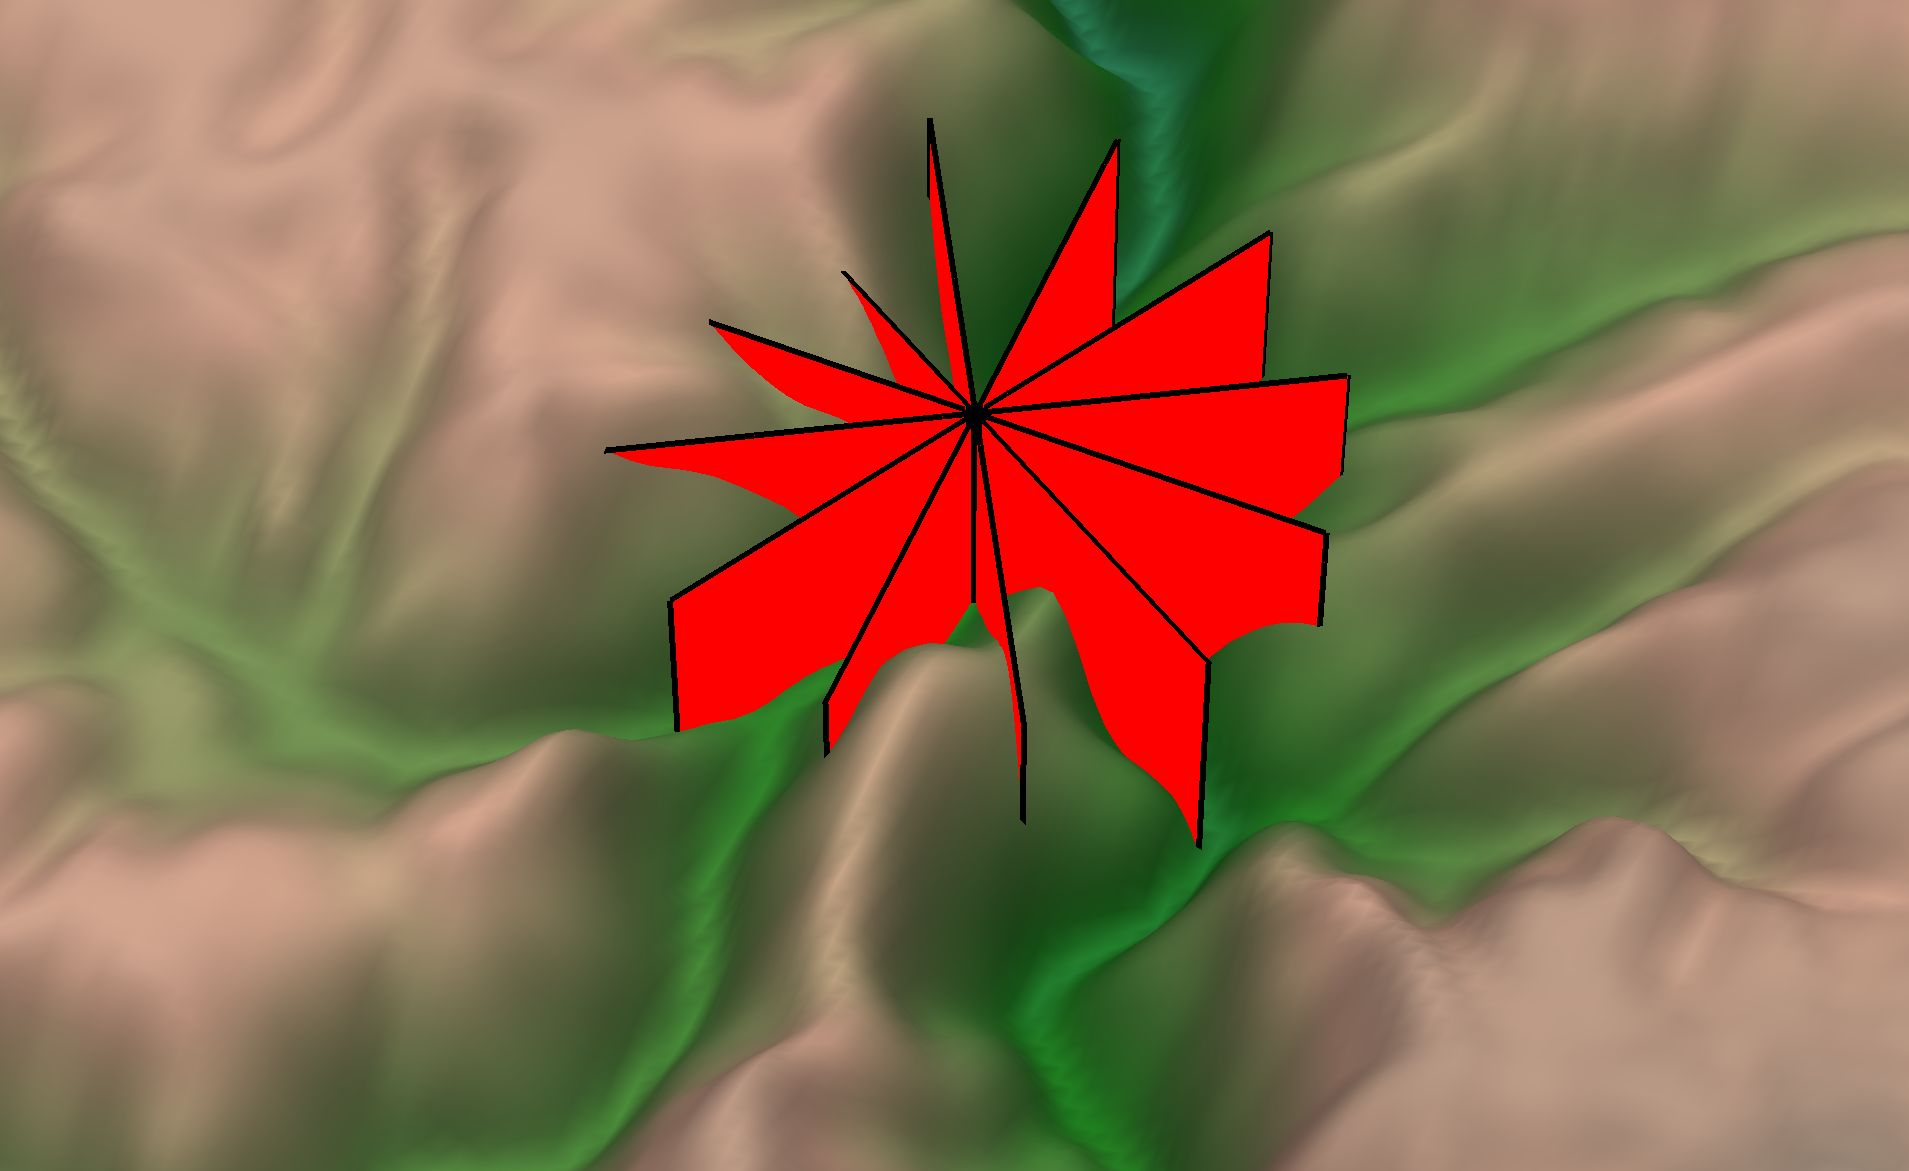
\includegraphics[width=0.99\linewidth]{images/crossSection.jpg}  \end{minipage}
  \begin{minipage}{0.49\linewidth} 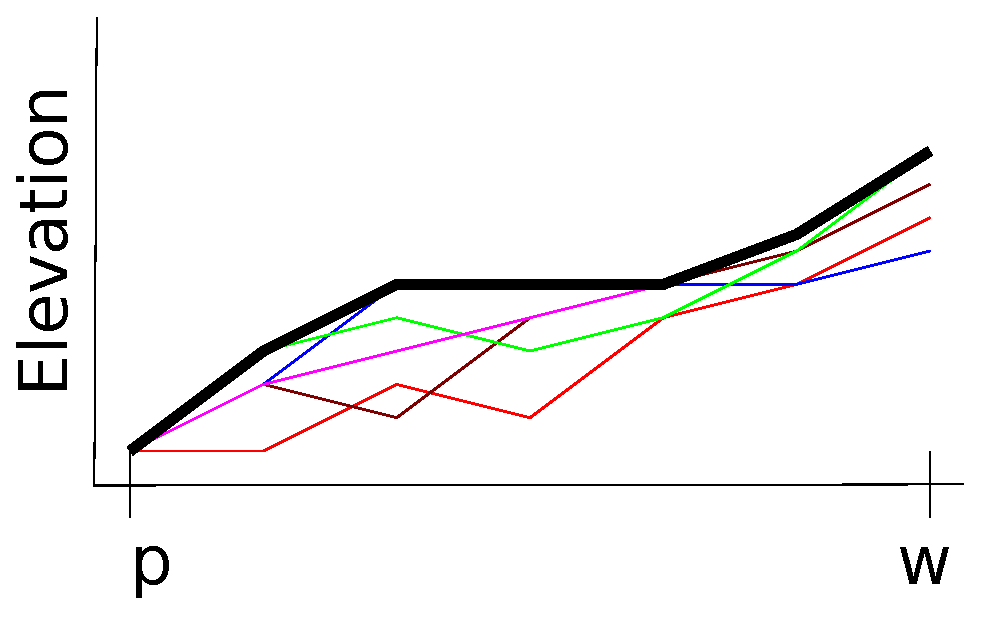
\includegraphics[width=0.99\linewidth]{images/CrossSections_2.eps} \end{minipage}
\end{center}
\caption[A visualization of the process of determining the union of the cross sections of the terrain's channels]{\label{figure:cross_section} A visualization of the process of determining the union of the cross sections of the terrain's channels. The left image depicts the process of gathering the cross sections. Each red plane is a cutting plane, and the cross section of the terrain determined by each one is collected. The right image depicts finding the union of all cross section. The colored thin lines represent the set of all cross sections at pixel $\bf{p}$, each one a collection of elevations of length $w$. The thick black line represents the final union.  }
\end{figure}

At each pixel $\textbf{p}_{i}$, a set of $c$ uniformly-spaced cross sections of the terrain are collected, where $c$ is an adjustable parameter. In this work, $c=120$ is an adequate value. This set of cross sections provides a profile of a channel at $c$ distinct angles. A sample of this procedure is shown in Figure \ref{figure:cross_section}. The cross sections span a distance $w$ from the center of $\textbf{p}_{i}$.
% , the second user-defined parameter to our system. 
The larger the value for $w$ is, the larger the area of influence on the terrain surface that is considered when determining the drill shape. For each pixel,
% in the channel network, 
uniformly spaced sample elevation points are collected in each direction along the crossing plane representing the cross section. Most of these sample points do not fall directly in the center of a pixel, and so simple bilinear interpolation is used to estimate the elevation of any sample point that does not exactly match a pixel center.

Once the set of cross sections is collected, its union is calculated by taking the maximum elevation value at each sampled distance from $\textbf{p}_{i}$, as depicted in Figure \ref{figure:cross_section}. This new terrain profile represents the widest that a drill can be in order to most accurately carve the terrain at $\textbf{p}_{i}$. 
The conservative estimate is necessary to guarantee that the terrain is not overly flattened by fitting a drill to a cross-section parallel to the channel length.
% , if the pixel is inside of a channel on the terrain.
Next, a curve is fit to the calculated union by treating the fitting as a constrained linear least-squares problem over the $w$ elevations of the union.
%  We constrain only the center point of the intersection, the elevation of $\textbf{p}_{i}$. The coefficients of this fitted quadratic equation represent the shape of the drill at $\textbf{p}_{i}$.
This fit curve can be of any family of functions the user desires. The coefficients of this function represent the encoding of the shape of the drill.
% , and are used to encode it.

% The terrain is completely represented by the list of pixels in the channel network and their associated drill's quadratic coefficients.


\subsection{Terrain Regeneration}

To regenerate the terrain from the drill representation, begin with a flat plateaued terrain of elevation $m$, where $m$ 
is the maximum elevation of $T$. A new terrain is procedurally generated by iteratively applying operations to this initial plateau, $T_{0}$. 
The $i^{th}$ 
drill
%, which corresponds with a pixel $\textbf{p}_{i}$ in the channel network of $D$, 
is represented by a $2k + 1 \times 2k + 1$ matrix 
$D_{i}$, where $k$ is referred to as the drill's ``influence''. Essentially, this is how large of an area of the terrain each drill operation 
affects.
% , and is the third and final user-defined parameter to the system. 
The width and height of $D_{i}$ must be odd because it must have a ``center'' pixel.

In order to drill the terrain, $D_{i}$ is centered over pixel $\textbf{p}_{i}$. The procedural generation is defined in Equation \ref{equation:drill}:

\begin{equation}
\label{equation:drill}
  T_{i} = \min\left( T_{i-1}, D_{i} \right)
\end{equation}

\noindent where the $\min\left(\right)$ function operates over the $2k + 1 \times 2k + 1$ area of $D_{i}$ and outputs a new matrix of minimum values between the pixels of $D_{i}$ and corresponding pixels of $T_{i-1}$. The resulting terrain has been drilled, and the process is repeated for the next operation, until all drills have been applied.
% The results of this procedural generation can be seen in Figure \ref{figure:lowest_errors}.




\section{Measuring Terrain Distances}
\label{section:TerrainDistances}

% It is necessary to have 
A quantitative measure of the difference between two terrain datasets, specifically height fields, $T_{0}$ and $T_{1}$, is necessary 
in order to judge the accuracy of terrain compression schemes and data representations (such as the drill operator presented in Chapter \ref{chapter:DrillOperator}).
Therefore, the notion of \textit{terrain distance}, or \textit{terrain dissimilarity}, must be explored. This chapter will present a series of metrics that determine $d\left(T_{0}, T_{1}\right)$, the distance between two height field datasets.

\subsection{Description of Distance Metrics}
\label{section:DescriptionOfMetrics}

Traditional distance metrics for spatial datasets, such as terrain surfaces, include Root Mean Square Error (RMSE) and Slope Surface RMSE (SSRMSE). These metrics provide a measure of 
% precision and accuracy lost 
distance on a global scope but ignore what can be thought of as the ``important'' characteristics of terrain, such as the shape and behavior of watersheds and channel networks,
and have been used to judge the accuracy of compression schemes and terrain representations (Stookey et al. \cite{Stookey08parallelodetlap}).


RMSE measures the root of the average squared difference in heights across the terrain, as shown in Equation \ref{equation:RMSMetric}:

\begin{equation}
\label{equation:RMSMetric}
%   RMSE\left(T_{0}, T_{1}\right) = \sqrt{ \frac{\displaystyle\sum_{\textbf{p}\in T_{0}, \textbf{q} \in T_{1}}{ \left(\textbf{p}_{z} - \textbf{q}_{z} \right)^2 } }{ |T_{0}| } }
  RMSE\left(T_{0}, T_{1}\right) = \sqrt{ \dfrac{\displaystyle\sum_{x < X} \displaystyle\sum_{y < Y} { \left( T_{0}\left(x,y\right) - T_{1}\left(x,y\right) \right)^2 } }{ X * Y } }
\end{equation}

\noindent where $X$ and $Y$ are the dimensions of $T_{0}$ and $T_{1}$, $T_{0}\left(x, y\right)$ is the elevation value at position $\left(x, y\right)$.
% , and 
% $z_{max}$ and $z_{min}$ are the maximum and minimum elevations of the pixels of $T_{0}$. 
% $|T_{0}|$ is the number of pixels in $T_{0}$.
This metric provides a single global distance measurement when comparing two datasets.
% , normalized by the value range of the pixels in $T_{0}$.

% % % For any two sets of pixels (in this case, the sets of all pixels in the channel network of each terrain), AHD finds  the maximum value of the average of the infimum of the
% % % distances between the sets,
% % % % the average of the shortest distance between their pixels, 
% % % as shown in Equation \ref{equation:hausdorffAvg}:
% % % 
% % % \begin{equation}
% % % \label{equation:hausdorffAvg}
% % % d_{ave} \left( N^{T_{0}}_{\tau}, N^{T_{1}}_{\tau} \right) = \max\left\{ \overline{\inf_{\textbf{p}_{j} \in N^{T_{1}}_{\tau}, \textbf{p}_{i} \in N^{T_{0}}_{\tau}} d\left(\textbf{p}_{i}, \textbf{p}_{j}\right)}, \overline{\inf_{\textbf{p}_{i} \in N^{T_{0}}_{\tau}, \textbf{p}_{j} \in N^{T_{1}}_{\tau}} d\left( \textbf{p}_{i}, \textbf{p}_{j} \right)} \right\}
% % % \end{equation}
% % % 
% % % \noindent where $N^{T_{0}}_{\tau}$ is the $i^{th}$ pixel of the set of channel network pixels extracted using threshold $\tau$, and $d\left( \textbf{p}_{i}, \textbf{p}_{j} \right) $ is
% % % the Euclidean distance between pixels $\textbf{p}_{i}$ and
% % % $\textbf{p}_{j}$. 
% % %  This metric tends to give a much more
% % % realistic look at the channel networks' distances.
% 
% 

% The slope surface RMSE metric measures the RMSE in the slope values at each pixel. To measure the SSRMSE, a slope surface is created by measuring the slope at each pixel. For each pixel $\textbf{p}_{i} = \left(x_{i}, y_{i}\right)$, the slope values is determined by Equation \ref{equation:PixelSlopeValue}:
% 
% \begin{equation}
% \label{equation:PixelSlopeValue}
%   \Delta_{xy} \left( \textbf{p}_{i} \right) = \dfrac{ |\left( \left( x_{i} + 1, y_{i}\right)_{z} - \left(x_{i} - 1, y_{i} \right)_{z} \right)| + |\left( \left( x_{i}, y_{i} + 1\right)_{z} - \left(x_{i}, y_{i} - 1 \right)_{z} \right)| }{2}
% \end{equation}
% 
% SSRMSE measures the RMSE between the slope surfaces of $T_{0}$ and $T_{1}$, $S_{T_{0}}$ and $S_{T_{1}}$, respectively. This is described in Equation \ref{equation:SSRMSE}
% 
% \begin{equation}
% \label{equation:SSRMSE}
%   SSRMSE\left(T_{0}, T_{1}\right) = RMSE\left(S_{T_{0}}, S_{T_{1}}\right)
% \end{equation}


RMSE provides a measure of elevation error, but oftentimes the more important characteristic of the terrain is the overall shape of the surface. Its shape determines the terrain's hydrography information, as well. The following metrics provide quantitative measurements of the dissimilarity between terrain shapes.

The gradient of the surface at each pixel is the determining factor in the flow of water across the terrain. Therefore, it is useful to measure the distance between the shapes of two terrain surfaces. In this work, the slope defined by Zevenberger-Thorne \cite{ESP:ESP3290120107} and the method presented by Tracy \cite{Tracy:2009:PPS:1751402} is used as a measure of slope dissimilarity. This measure requires finding the vector normal to the surface at each pixel (the vector perpendicular to the gradient direction, or tangent, of the surface). The normal at each corresponding pixel is found, and the angle between the vectors is measured. The average of these angles across the entire terrain provides a value for the distance, $SSE\left(T_{0}, T_{1}\right)$.

% 
% \begin{equation}
%   SSE\left(T_{0},T_{1}\right) = 
% \end{equation}



Both SSE and RMSE provide a measure of global distances between two spatial datasets. However, when measuring the distance between two terrain datasets, it is often more appropriate to determine how dissimilar specific characteristics of the terrain are from one another.

The following metrics take as input two channel networks
($N^{T_{0}}_{\tau}$ and $N^{T_{1}}_{\tau}$) and return the distance between
them. These metrics are used to help define the difference between the
terrains and thresholds from which the networks result. 
% % Since the metrics have been designed to 
% % take in any channel networks, comparisons between terrains
% % from simulation data (different time steps in the same sequence), between unrelated terrains, or even
% the same terrain with networks formed using different thresholds are possible.

% \subsection{Pixel-to-Pixel Correspondence Metric}
% \label{section:PixelToPixelCorrespondence}

The first metric is the pixel to pixel correspondence metric, described in equation \ref{equation:pix_dist}, in which
each pixel of $N^{T_{0}}_{\tau}$ is compared to each in $N^{T_{1}}_{\tau}$,
and two pixels are said to correspond if 
% their addresses have the same length (meaning 
they are each the same depth in their respective networks,
and their flow travels in the same direction. 
% I do not compare
% addresses directly because of potential inconsistencies in the
% labeling scheme applied to two similar but not identical networks.
% A slight change in threshold can cause a new, very small network to
% form elsewhere in the terrain, and as a result the ID system for the
% networks (Figure \ref{figure:addressingScheme}) is not comparable
% between thresholds, only a pixel's position within its own network.

\begin{align}
\label{equation:pix_dist}
  d_{pix} \left( N^{T_{0}}_{\tau}, N^{T_{1}}_{\tau} \right) = \dfrac{ \left| \left\{ \textbf{p}_{i} \  | \ \textbf{p}_{i} \rightarrow \textbf{p}_{j} \right\} \right| }{ \left| N^{T_{0}}_{\tau} \right|  }
\end{align}

\noindent where $\textbf{p}_{i} \in N^{T_{0}}_{\tau}\,$ and
$\textbf{p}_{j} \in N^{T_{1}}_{\tau}$ is its corresponding pixel (same x,
y coordinates in its respective terrain), and $\left| N^{T_{0}}_{\tau}
\right|$ is the total number of pixels compared, a normalizing
component.

% One major shortcoming of the pixel-to-pixel correspondence metric is that a small change in the network downstream of any pixel has the potential to drastically change the address assigned to the pixel. For this reason, the use of this metric should be limited to major channel networks after a pruning procedure has taken place. Thus, 
Pixels of similar networks correspond regarding their positions in the network, and thus this metric is a normalized count of the number of correlated pixels between two networks. This metric also inherently uses channel length as a measure of dissimilarity.

% \subsection{Hausdorff Distance Metrics}citeulike:1146653
% \label{section:HausdorffDistanceMetrics}

The second metric is an adaptation of the traditional \emph{Hausdorff distance} metric, defined in equation \ref{equation:hausdorff}.

\begin{align}
\begin{split}
\label{equation:hausdorff}
& d_{haus} \left( N^{T_{0}}_{\tau}, N^{T_{1}}_{\tau} \right) =  
\max \left\{ \sup_{ \textbf{p}_{i} \in N^{T_{0}}_{\tau} } \inf_{ \textbf{p}_{j} \in N^{T_{1}}_{\tau} } d\left( \textbf{p}_{i} \, \textbf{p}_{j} \right) \, \sup_{ \textbf{p}_{j} \in N^{T_{1}}_{\tau} } \inf_{ \textbf{p}_{i} \in N^{T_{0}}_{\tau} } d\left( \textbf{p}_{i} \, \textbf{p}_{j} \right) \right\}
%  \max\left\{ \overline{\inf_{\textbf{p}_{j} \in N^{T_{1}}_{\tau}, \textbf{p}_{i} \in N^{T_{0}}_{\tau}} d\left(\textbf{p}_{i}, \textbf{p}_{j}\right)}, \overline{\inf_{\textbf{p}_{i} \in N^{T_{0}}_{\tau}, \textbf{p}_{j} \in N^{T_{1}}_{\tau}} d\left( \textbf{p}_{i}, \textbf{p}_{j} \right)} \right\}
\end{split}
\end{align}

\noindent where $d\left( \textbf{p}_{i}, \textbf{p}_{j} \right) $ is
the Euclidean distance between pixels $\textbf{p}_{i}$ and
$\textbf{p}_{j}$. The Hausdorff distance metric is a measure over all of the pixels in each channel network. It is defined as the maximum distance of the set of minimum distances between a pixel $\textbf{p}_{i}$ in $N^{T_{0}}_{\tau}$ and the pixels in $N^{T_{1}}_{\tau}$. However, due to the nature of the metric, it can lend too much weight to outliers. Therefore, a third metric, the average Hausdorff distance as proposed by Dubuisson and Jain \cite{citeulike:1146653}, is used.

For any two sets of pixels, the average Hausdorff metric finds the average of the shortest distance between their respective pixels, as shown in Equation \ref{equation:hausdorffAvg}:
%  the average Hausdorff distance metric, as described by Equation \ref{equation:hausdorffAvg}.

\begin{align}
\label{equation:hausdorffAvg}
\begin{split}
& d_{avg} \left( N^{T_{0}}_{\tau}, N^{T_{1}}_{\tau} \right) = 
% \max \left\{ \overline{ \inf_{\textbf{p}_{j} \in N^{T_{1}}_{\tau} \textbf{p}_{i} \in N^{T_{0}}_{\tau} } d\left( \textbf{p}_{i}, \textbf{p}_{j} \right) }, \overline{ \inf_{\textbf{p}_{i} \in N^{T_{0}}_{\tau}, \textbf{p}_{j} \in N^{T_{1}}_{\tau} } d\left( \textbf{p}_{i}, \textbf{p}_{j} \right) } \right\}
 \max\left\{ \overline{\inf_{\textbf{p}_{j} \in N^{T_{1}}_{\tau}, \textbf{p}_{i} \in N^{T_{0}}_{\tau}} d\left(\textbf{p}_{i}, \textbf{p}_{j}\right)}, \overline{\inf_{\textbf{p}_{i} \in N^{T_{0}}_{\tau}, \textbf{p}_{j} \in N^{T_{1}}_{\tau}} d\left( \textbf{p}_{i}, \textbf{p}_{j} \right)} \right\}
\end{split}
\end{align}

\noindent where 
$\textbf{p}_{i} \in N^{T_{0}}_{\tau}$ is the $i^{th}$ pixel of the set of channel network pixels 
of $T_{0}$ extracted using threshold $\tau$, $N^{T_{0}}_{\tau}$. The overline means ``mean value of''. 
It is important to note that AHD is limited to the channel networks of the terrain, whereas RMSE is applied globally. 
Limiting RMSE to only $N_{\tau}$ would not give an accurate picture of how close the terrains' hydrography networks are, 
since the network pixels are found by looking at the global flow pattern. Even if the elevations of the pixels in $N_{\tau}$ 
are comparable, it does not indicate that the overall terrain shape is similar. In addition, slight variations 
in the location of the pixels in $N_{\tau}$ would render RMSE unusable.

% \noindent or the maximum value of the average of the infimum of the
% distances between the sets. This metric tends to give a much more
% realistic look at the channel networks' distances, as it smooths out inaccurate distances created by outliers. 


The average Hausdorff distance provides a general picture of how close the pixels in $N^{T_{0}}_{\tau}$ are to those in $N^{T_{1}}_{\tau}$. It is important to note that this is a Euclidean metric, based on their exact positions in $\mathbb{R}^{3}$. All information regarding the geometry of the channel network (such as slope), meander, or flow is ignored. However, unlike the RMS Error metric, the average Hausdorff distance is a measurement of the geometric distance between only the pixels in the channel network, and thus it places emphasis on them and ignores the rest of the terrain. In this way, ``unimportant'' elevation information and outliers are not taken into account. By limiting the metric to pixels in the channel network, the geometry of the entire terrain is inherently incorporated but weighted by distance and contribution to the channel network.
% , because it is all data critical to the formation of the channel network, while focusing the metric on the important pixels.

Another hydrography-specific metric employed in this thesis is the Ridge-River metric, proposed by Muckell et al. \cite{Muckell:2009:EHP:1517463.1517470}, $d_{RR}$. This metric measures the error in the overall structure of the flow network of a regenerated terrain by measuring the energy required by water to flow across the original terrain $T_{0}$ given the flow directions for the pixels in $T{1}$. In essence, the metric measures how poorly the flow network of $T_{1}$ fits $T_{0}$ when overlayed on top of it. Two separate energies are calculated: the total flow uphill, and the total flow downhill. These can be written as:

\begin{align}
  \label{equation:EnergyDown}
  EnergyDown & = \displaystyle\sum_{x < X} \displaystyle\sum_{y < Y} \text{max} \left( 0, T_{0}\left(x,y\right) - T_{0}\left(r\left(x,y\right)\right) \right) * flowAccum_{\left(x,y\right)} \\
  EnergyUp & = \displaystyle\sum_{x < X} \displaystyle\sum_{y < Y} \text{max} \left( 0, T_{0}\left(r\left(x,y\right)\right) - T_{0}\left(x,y\right) \right) * flowAccum_{\left(x,y\right)} \\
%   d_{RR} & = 
% 
%   EnergyDown & = \displaystyle\sum_{\textbf{p}\in T_{0}, \textbf{q} \in T_{1}} \text{max}\left( 0, E_{i} - E_{r\left(i\right)} \right) * flowAccum_{i} \\
%   EnergyUp & = \displaystyle\sum_{\textbf{p}\in T_{0}, \textbf{q} \in T_{1}} \text{max}\left( 0, E_{r\left(i\right)} - E_{i}  \right) * flowAccum_{i} \\
  d_{RR} \left( N^{T_{0}}_{\tau}, N^{T_{1}}_{\tau} \right) & = \dfrac{EnergyUp}{EnergyDown}
\end{align}

\noindent where $r\left(x,y\right)$ is the pixel that receives flow from pixel $\left(x,y\right)$ on $T_{1}$. The energies are calculated by summing the measured elevation increase for water flowing uphill (or downhill for $EnergyDown$), weighted by the total flow accumulation of pixel $\left(x,y\right)$ on $T_{1}$. 

Because the method for extracting $T_{0}$'s hydrography results in some uphill flow, $d_{RR}$ is calculated for the original terrain's hydrography network as well. This value is subtracted from $T_{1}$'s $d_{RR}$ for the final error measurement, thus providing a measure of how much hydrography error is introduced by the regeneration.


\subsection{Finding an Optimal Flow Threshold}

Once a definition of the distance between two terrains has been determined, then an optimal threshold value that minimizes the distance between two terrains can be found. 
% 
% A good deal of work has been done with the intent of finding an \emph{optimal} flow accumulation value with which to threshold the flow accumulation matrix to extract the channel network. 
There have been attempts to use drainage density (a ratio of flow value to pixel watershed size) as a value to threshold instead of flow accumulation, while others have attempted to use local curvature or gradient values, as discussed in section \ref{section:ChoosingAFlowThreshold}. 


A simple brute force method will find this threshold among a set of terrains, by trying several different thresholds for the terrains in question and recording those that produce the smallest distances.
What is a more interesting challenge is finding the optimal threshold to apply to each terrain in a sequential series. 
If there are several terrains that belong to a series (such as time steps in an erosion simulation, or several regenerated terrains that had been compressed with various parameters), $\{ T_{i} \}$, finding an optimal threshold to compare their channel networks requires a degree of sequential coherence so that networks change smoothly as one moves from one terrain to another.
% 
% 
% It is clear that this is an interesting and important avenue of research. With this in mind, I introduce 
% Therefore, a method for finding the optimal flow threshold with which to compare two terrains, $T_{i}$ and $T_{j}$ in a sequence is introduced.
% representing sequential time steps, $D_{i}$ and $D_{j}$, in a series of datasets from our erosion simulation. This procedure is limited to this situation because of the limited nature of the metrics presented in section \ref{section:DescriptionOfMetrics}. Because they apply best when two terrains should match closely with only minute differences, comparing two sequential datasets is an ideal situation.
% This algorithm works best when the extracted channel networks are similar to one another, such as when testing the accuracy of a compression scheme.

Despite the fact that $T_{i}$ and $T_{j}$ are assumed to be similar, the extracted channel networks are very sensitive to small changes in the chosen threshold value. Given this, the same threshold cannot necessarily be applied to $T_{i}$ and $T_{j}$, as there is no guarantee that the result channel networks will resemble one another.
%  (ADD IMAGE)
Additionally, when measuring the dissimilarity between a decompressed terrain and its baseline, small elevation errors may result in the same threshold resulting in significantly different channel networks. Therefore, a method for choosing threshold values for each terrain is important. 
% For the time being, I restrict its use to a series of temporally adjacent terrains in a series of time steps.

A moving window algorithm that can use any of the metrics introduced in section \ref{section:DescriptionOfMetrics} to determine the threshold that minimizes the distance between $T_{i}$ and $T_{j}$ is shown in algorithm \ref{algorithm:idealThreshold}.

\begin{algorithm}[t]
\begin{algorithmic}
  \STATE $avg \gets 0$
  \STATE $nComparisons \gets 0$
    \FOR{$w_{cur} = t - \mbox{\em WINDOW} \to t + \mbox{\em WINDOW}$}
      \FOR{$\tau = \tau_{min} \to \tau_{max}$}
	  \STATE $dist \gets d\left( N^{t}_{\tau}, N^{w_{cur}}_{\tau} \right)$
	  \STATE $avg \gets avg + \tau * c\left( dist \right)$
	  \STATE $nComparisons \gets nComparisons + 1$
     \ENDFOR
  \ENDFOR
  \STATE $avg \gets avg / nComparisons$
  \STATE return $avg$
\end{algorithmic}
\caption[The moving window algorithm for finding the ideal threshold.]{\label{algorithm:idealThreshold} The moving window algorithm for finding the ideal threshold between two terrains by comparing its channel network with those of its neighbors. {\em WINDOW} is a constant window size, $d\left(N^{t}_{\tau}, N^{w_{cur}}_{\tau} \right)$ is the distance between channel networks $N^{t}_{\tau}$ and $N^{w_{cur}}_{\tau}$, $[ \tau_{min}$, $\tau_{max} ]$ is the range of threshold values we wish to test, and $c\left( dist \right)$ is a weight applied to the distance between networks. A window size of 2 worked well for a 10-terrain sequence, and for $c$, a weight of 1 is often sufficient.}
\end{algorithm}

This method is limited by the nature of the windowing algorithm. Possible thresholds are tested across neighbors, but the sequential coherence may be adversely affected by the neighbors' choice for its threshold. 
% This windowing algorithm was used to determine the optimal thresholds to use 








% \chapter{Using the Drill Operator}
% \label{chapter:UsingTheDrillOperator}
% 
% The drill operator presented in chapter \ref{chapter:DrillOperator} provides a unique and novel method for representing the shape of a terrain surface. This chapter explores the operator's utility 
% by presenting various enhancements, applications, and uses for the drill operator with regard to accurately and compactly representing terrain data.
% % by presenting accuracy tests that show how closely the operator representation can mimic terrain data. These initial accuracy tests are followed by an in depth exploration of various expanded uses and applications of the drill operator.


\section{Initial Accuracy Trials}
\label{section:DrillAccuracyTests}

To determine the feasibility of representing terrain as drills, initial accuracy tests were performed to determine how closely the drill representation modeled the $400 \times 400$ mountainous dataset seen in Figure \ref{figure:mtn2_original}. All tests were performed in Ubuntu 11.04 with a quad-core AMD Phenom II X4 945 Processor, with 8GB of RAM. The code was written in MATLAB.

\subsection{Experimental Methodology}

The three parameters of the system, as described in Chapter \ref{chapter:DrillOperator}, are the threshold used to extract the original terrain's channel network $\tau$, the size of the cross section $w$, and the influence of a drill (size of the representative matrix) $k$. Each of 3 thresholds, 3 cross-section sizes, and 6 influence values were used to build regenerated terrains in the factorial experiment described in this section. 

For each set of parameter values, the total error between the generated terrain and the initial terrain was calculated using a measure for dissimilarity between the two sets.
These metrics take as input two channel networks
($N^{i}_{\tau}$ and $N^{j}_{\tau}$) and return the distance between
them.
 The two metrics used were the standard root mean squares error (RMSE) metric, and the averaged Hausdorff distance (AHD) metric as described in Section \ref{section:DescriptionOfMetrics}.
% by Stuetzle et al. \cite{stuetzle-TerrainDistances}, inspired by the shape analysis techniques discussed in Section \ref{section:ShapeAnalysisTechniques}.

It is important to note that AHD is limited to the channel networks of the terrain, whereas RMSE is applied globally. Limiting RMSE to only $N_{\tau}$ would not give an accurate picture of how close the terrains' hydrography networks are, since the network pixels are found by looking at the global flow pattern. Even if the elevations of the pixels in $N_{\tau}$ are comparable, it does not indicate that the overall terrain shape is similar. In addition, slight variations in the location of the pixels in $N_{\tau}$ would render RMSE unusable. Therefore, the results for both metrics are analyzed in context of their maximum error and what they mean from a physical standpoint.

\subsection{Results and Discussion of Initial Accuracy Trials}
\label{section:DrillAccuracyResultsAndDiscussion}

\begin{figure}
\begin{center}
  \begin{minipage}{0.49\linewidth}
     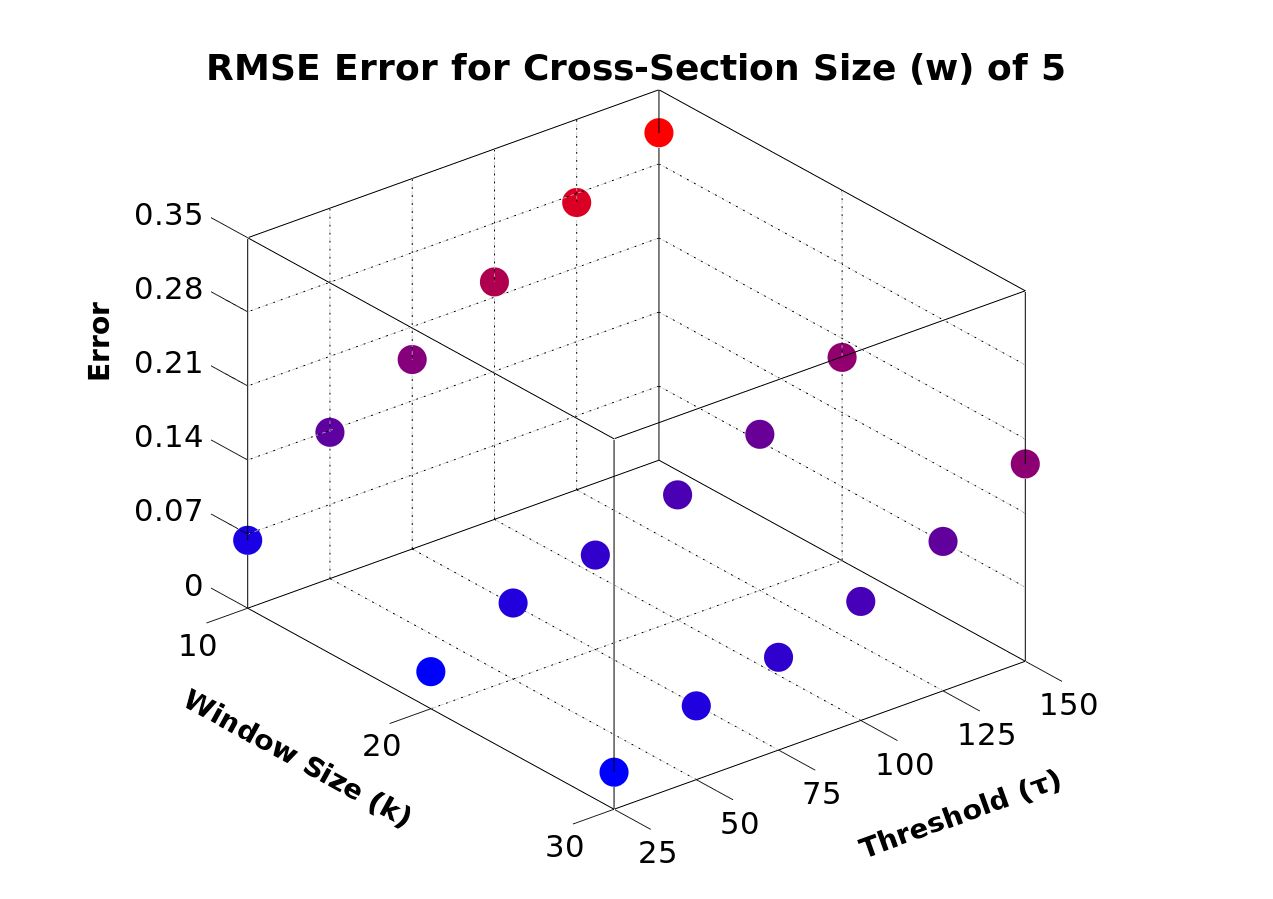
\includegraphics[height=0.25\textheight,width=0.99\linewidth]{images/RMSE_Graph_CS5.jpg} 

     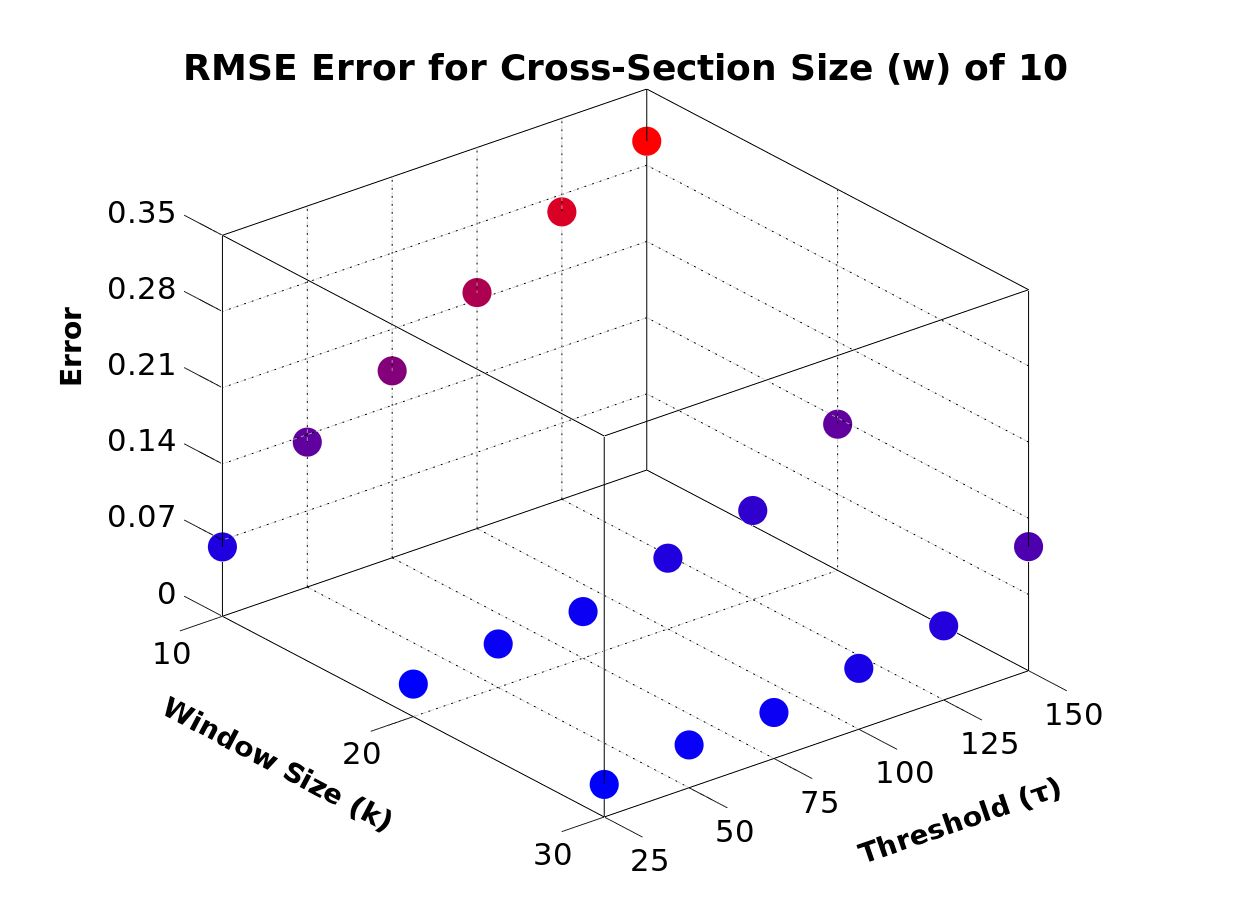
\includegraphics[height=0.25\textheight,width=0.99\linewidth]{images/RMSE_Graph_CS10.jpg}

     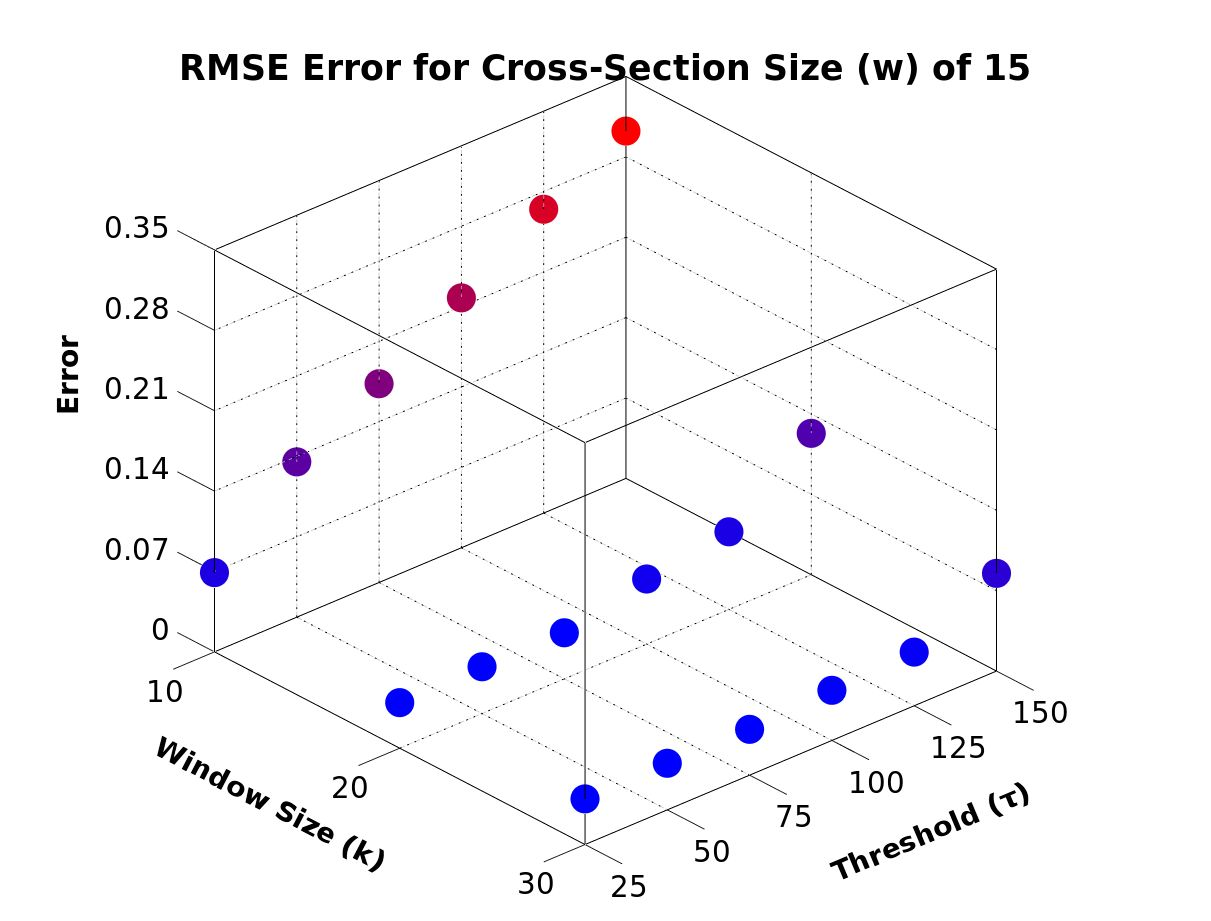
\includegraphics[height=0.25\textheight,width=0.99\linewidth]{images/RMSE_Graph_CS15.jpg}  
  \end{minipage}
  \begin{minipage} {0.49\linewidth} 
    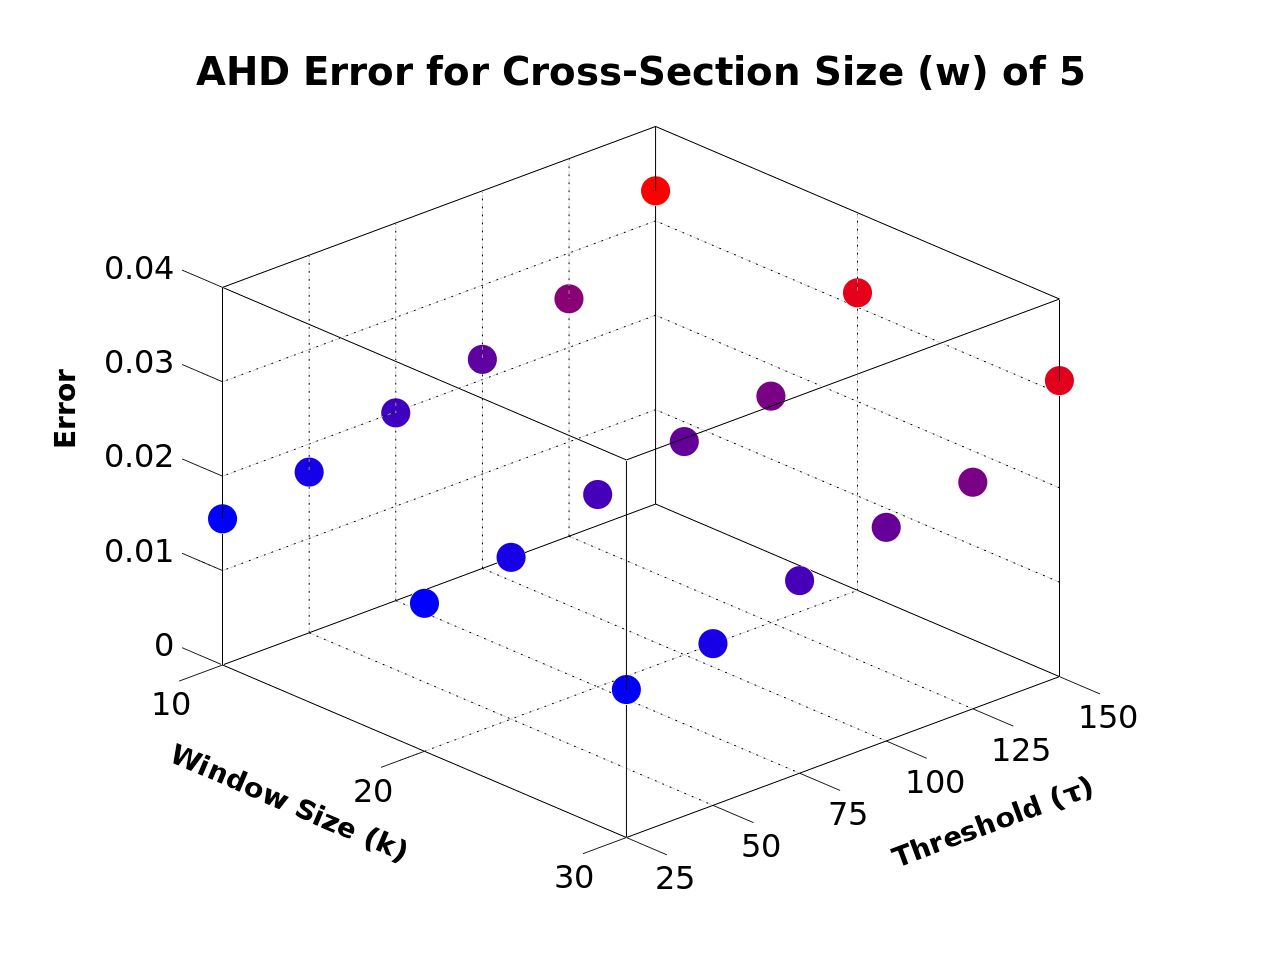
\includegraphics[height=0.25\textheight,width=0.99\linewidth]{images/AHD_Graph_CS5.jpg} 
 
    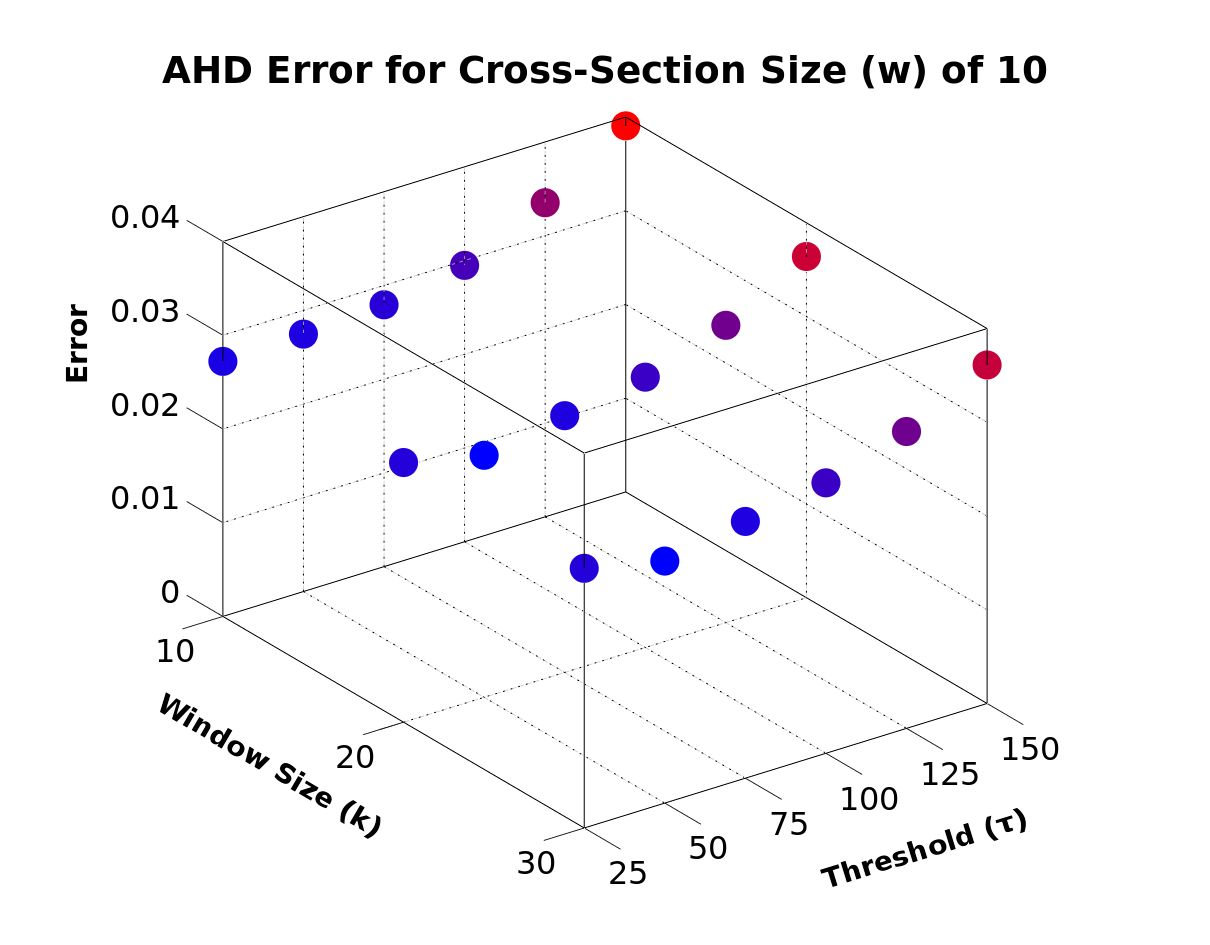
\includegraphics[height=0.25\textheight,width=0.99\linewidth]{images/AHD_Graph_CS10.jpg}

    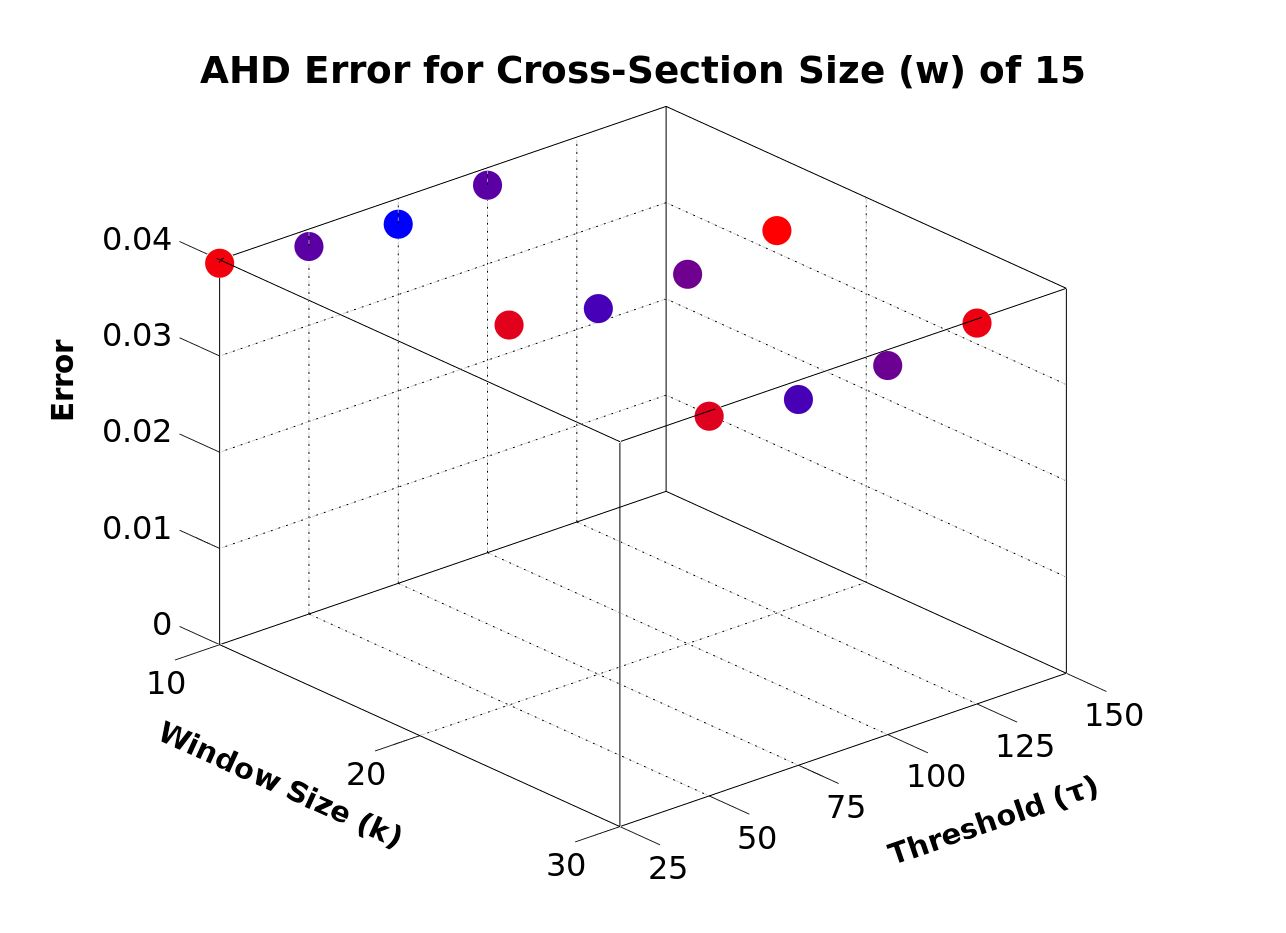
\includegraphics[height=0.25\textheight,width=0.99\linewidth]{images/AHD_Graph_CS15.jpg}
  \end{minipage}
\end{center}
\caption[The results for the concept tests for the drill operator]{\label{figure:results} The results of accuracy testing. The left column depicts the error measured using the RMSE metric, and the right column depicts error measured used the AHD metric. Each row shows a different value for the cross section window size (parameter $w$). Each metric's data is normalized. Red indicates high error, whereas blue indicates low error, local to each dataset.
\fbox{FIX LATER}}
\end{figure}


\begin{figure}[t]
\begin{center}
  \begin{minipage}{0.49\linewidth} 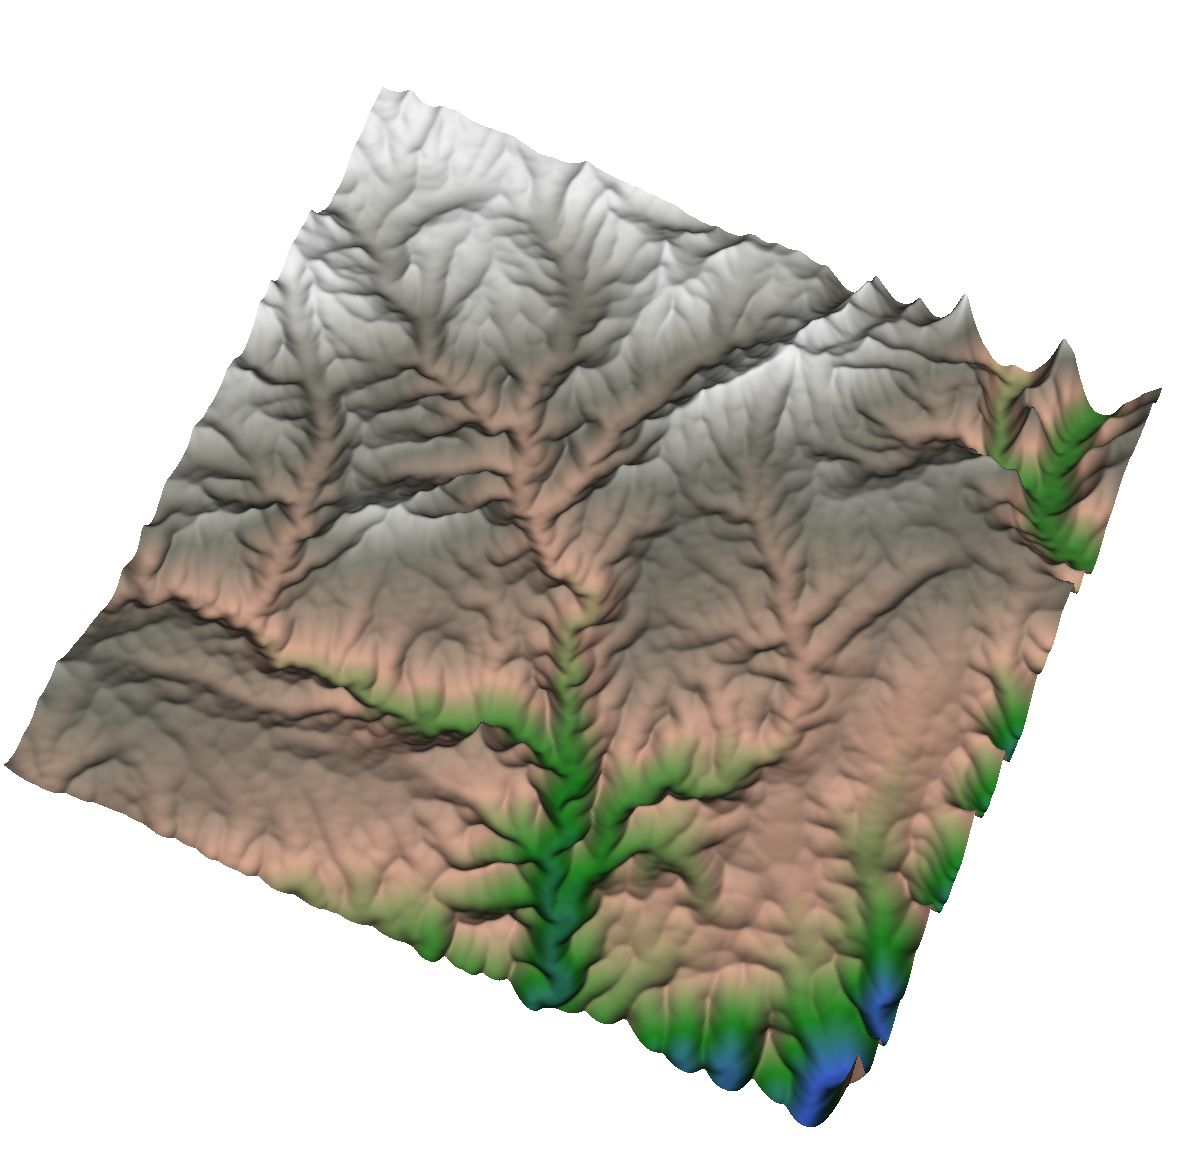
\includegraphics[width=0.99\linewidth]{images/W10_I20_T25.jpg} \\ \centering $\tau=25$, $w=10$, $k=20$ \end{minipage}
  \begin{minipage}{0.49\linewidth} 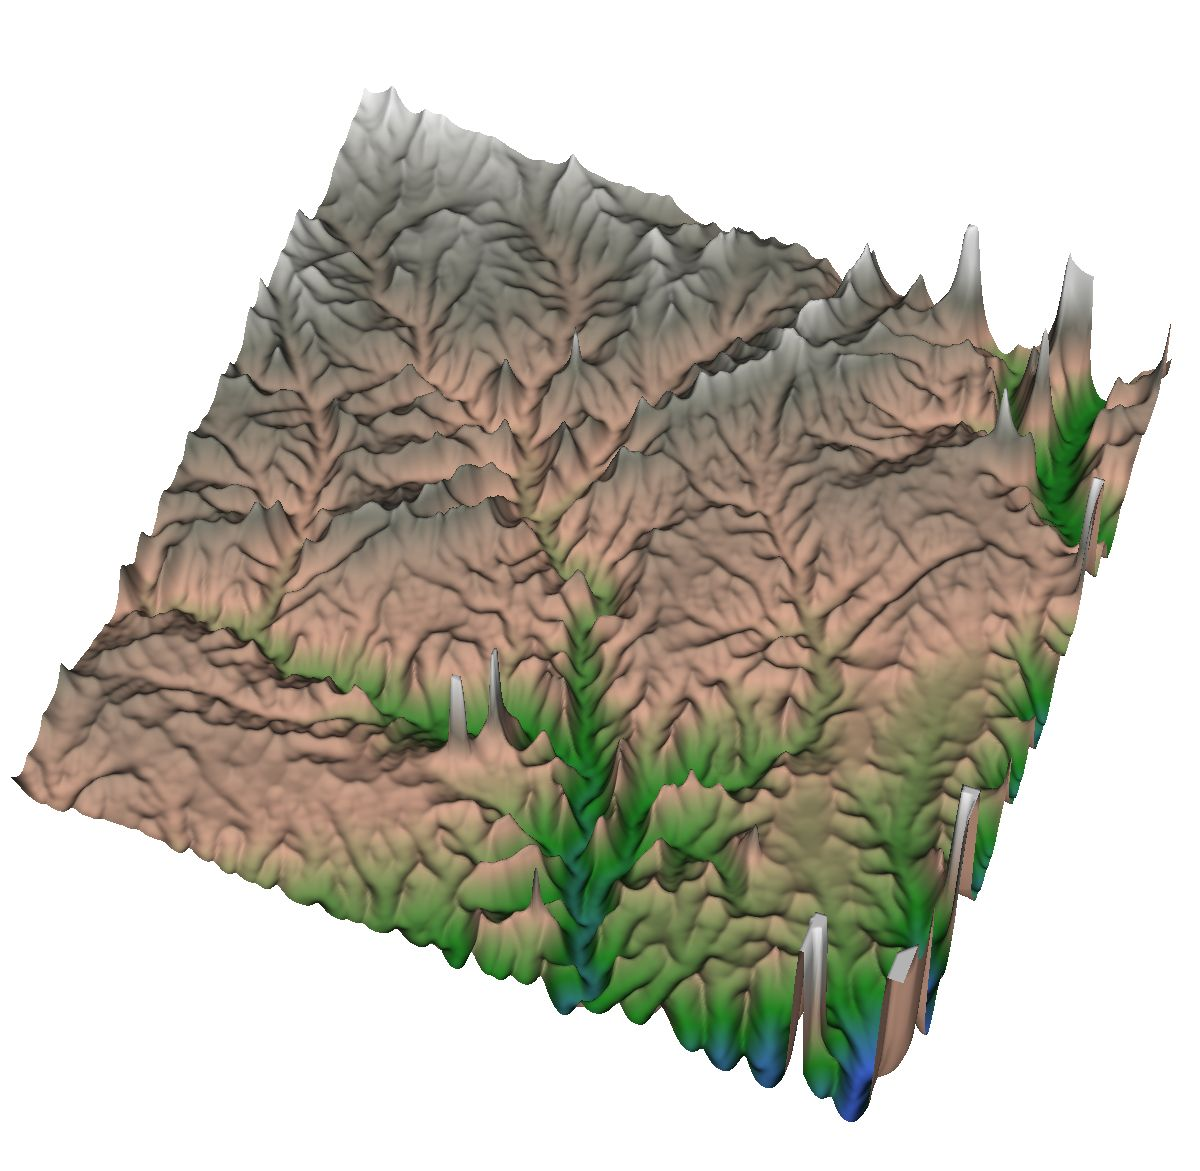
\includegraphics[width=0.99\linewidth]{images/W5_I10_T25.jpg} \\ \centering $\tau=25$, $w=5$, $k=10$ \end{minipage}
\end{center}
\caption[Regenerated terrains with lowest errors]{\label{figure:lowest_errors} The left image depicts the regenerated terrain with the lowest RMSE value, and the right image depicts the regenerated terrain with the lowest AHD error. The parameters responsible for the terrain are listed below the images. }
\end{figure}


The results for the accuracy tests are provided in Figure \ref{figure:results}. The left column of Figure \ref{figure:results} presents the data for the RMSE metric, and the data for the AHD is on the right. The error divisor for RMSE was the total elevation range of the original terrain, whereas the error divisor of AHD was the distance between pixel 0,0 and pixel $n$,$n$, the corners of the terrain. Since elevation is ignored for this divisor, it is possible for AHD error be greater than 1.0. 

$\tau$ values of 25 created considerably denser channel networks than $\tau$ values above 100, and so they are both more accurate and take considerably longer to calculate. The two channel networks can be seen in Figure \ref{figure:mtn2_original}. For reference, the maximum flow value for a pixel in the dataset is 102,245, and a threshold of 25 resulted in a channel network with $\approx19,000$ pixels, whereas a threshold of 100 resulted in a network of $\approx12,000$ pixels. Calculating the drill representation of a terrain with a flow threshold of 25 took approximately three minutes, and times decreased linearly with the increase in threshold value. The time for regenerating the terrain from the drill representation was quicker by approximately a factor of ten. It is important to note that optimization was not a focus at this time, and there exist many techniques that will be utilized in the future to reduce the time the algorithm takes.

There are several observations to be made regarding the accuracy data. The first is that, with ``good'' parameters (meaning none that create outliers in the error data), the accuracy is actually quite high with regard to both RMSE and AHD metrics, between 0.015 and 0.025. As with any algorithm, there is a trade-off between time and accuracy. The lower the threshold, the more pixels in the hydrography network, and so the slower the process, but the more accurate the results become. This is true in every case, and it makes intuitive sense. 

$\tau$ is the most influential parameter with regard to both metrics. 
This makes sense, since the drill is centered around the pixels of $N^{i}_{\tau}$. 
% shape calculation is constrained to pass through the center of $N^{i}_{\tau}$. 
Because AHD measures how close the channel networks are to one another, the more pixels there are in the channels the more likely it is that the channel networks overlap. By nature of the AHD, this will result in very low error. If the channel network is not dense enough, then the drill may not reach much of the terrain at all, and so the RMSE is also very much influenced by the value of $\tau$. More interesting is that the minimum RMSE occurred for when $w = 10$ and $k = 20$. It makes sense that a drill will need some influence over the area around the channel in order to reduce the RMSE, because without it there would be large areas of the terrain untouched by any drill, adding considerably to the overall error (that AHD would ignore). 

From a purely visual standpoint, many of the terrains pass the eyeball test. A side-by-side comparison of the terrains that represent the lowest error for each of the metrics is found in Figure \ref{figure:lowest_errors}. Notice is that the channels do seem to be somewhat wider in the RMSE winner, whereas they are more pointed, but areas of the terrain are missed by drills completely, in the AHD winner. Interestingly, the left image in Figure \ref{figure:lowest_errors} is one of the terrains we deem to be the most ``visually pleasing''. These often have higher $k$ and $w$ values, which may be a result of drills that flatten artifacts out of the terrain. This result demonstrates why, when choosing parameters for the drill operator, it is often smart to take both error metrics into account.


\section{Families of Functions for Drill Shape}
\label{section:FamiliesOfFunctions}

\begin{figure}[t]
  \caption[Graphical representations of drill shape functions.]{\label{figure:FamiliesOfFunctions} This figure shows graphical 2D examples of each of the families of functions making up several possible drill shapes.}
\end{figure}

\fbox{I will make a figure of the function families tested}


\begin{table}[t]
  \centering
  \begin{tabular}{ | c | c | c | c | }
    \hline
      & \textbf{AHD} & \textbf{RMSE} & \textbf{SSRMSE} \\
    \hline
    \textbf{Linear}&&&  \\
    \hline
    HILL1 & 0.0572 & 0.0700 & 0.1013 \\
    HILL2 & 0.1848 & 0.1564 & 0.0923 \\
    HILL3 & 0.0563 & 0.0394 & 0.0644 \\
    MTN1 & 0.0483 & 0.0517 & 0.1000 \\
    MTN2 & 0.0285 & 0.0141 & 0.0819 \\
    MTN3 & 0.0383 & 0.0379 & 0.0764 \\
    \hline
    \textbf{Quadratic}&&& \\
    \hline
    HILL1 & 0.0673 & 0.1230 & 0.1581 \\
    HILL2 & 0.1840 & 0.1581 & 0.1022 \\
    HILL3 & 0.0678 & 0.0965 & 0.1888 \\
    MTN1 & 0.0568 & 0.1364 & 0.2403 \\
    MTN2 & 0.0192 & 0.0184 & 0.1080 \\
    MTN3 & 0.0362 & 0.0771 & 0.1477 \\
    \hline
    \textbf{Cubic}&&&  \\
    \hline
    HILL1 & 0.2757 & 0.3413 & 0.3803 \\
    HILL2 & 0.1820 & 0.1674 & 0.0894 \\
    HILL3 & 0.2060 & 0.2412 & 0.3155 \\
    MTN1 & 0.6620 & 0.5032 & 0.1197 \\
    MTN2 & 0.0160 & 0.2521 & 0.1227 \\
    MTN3 & 0.5117 & 0.4783 & 0.1041 \\
    \hline
  \end{tabular}
  \caption[Minimum error values in tests for different drill shape function families.]{\label{table:FamiliesOfFunctionsResults} This table presents the minimum error found for each of RMSE, AHD, and SSRMSE metrics, divided by function family. The top third of the table refers to data for linear drill shapes, the middle third to quadratic drill shapes, and the bottom third to cubic drill shapes. The results for each of the six datasets found in Figure \ref{figure:SixDatasets} is reported.}
\end{table}

% Properly determining the drill shape can have a profound effect on the accuracy and flexibility of the operator. 
This section explores various drill shapes that can be used to represent the terrain surface.
The drill shape can be represented by any two-dimensional curve (not necessarily by a single-valued function). 
As a preliminary investigation into the effect of the drill shape, the following polynomial curves were investigated:
% This work investigates polynomial and logistic functions. 

\begin{itemize}
  \item Linear functions: Polynomials of degree one
  \item Quadratic functions: Polynomials of degree two
  \item Cubic functions: Polynomials of degree three
  \item Logistic functions
\end{itemize}

\fbox{FIX THE GRAPHIC}

\noindent Graphical examples of each of these families of functions can be seen in Figure \ref{figure:FamiliesOfFunctions}. Each family allows for arbitrarily steep slope (although slight modifications are required for vertical and negative slopes, though those can be incorporated with slight modifications to the fitting functions). 

A test was performed comparing the accuracy of each drill shape. Each test was a factorial experiment using the same three parameters described in Section \ref{section:DrillAccuracyTests} (channel network threshold, drill influence, cross-section size). For these experiments, the threshold was determined by the percentage of pixels to be extracted, and so $r$ was used as the third parameter in lieu of $\tau$. Using a percentage to define the extraction threshold provides a better idea of how much of the terrain is included in the channel network, and, more importantly, how many pixels are required to encode the terrain.

Three of the error metrics defined in Section \ref{section:DescriptionOfMetrics} were used for this test: AHD, RMSE, and SSRMSE. Beyond the fact that slope is an important terrain characteristic, the SSRMSE metric was included with AHD and RMSE (used in the test in Section \ref{section:DrillAccuracyTests}) in these tests because visual inspection of the results from Section \ref{section:DrillAccuracyResultsAndDiscussion} revealed that the peak areas between channels were pointed more than the original terrain. The slope-based metric will penalize this behavior more than RMSE.

Each possible drill function was tested in a factorial experiment. For each segment of the channel network, a single drill shape was determined (minimizing the number of fittings needed). Values up to 30 were tested for $r$ and $w$, and in the interest of limited time $k$ was set to the value of $w$. Logistic functions were immediately thrown away, as their results were incredibly bad. However, the results for the other three function families are presented in Table \ref{table:FamiliesOfFunctionsResults}.

Each of the values in the table is the minimum error found for each respective metric and dataset. Once again, the density of the pixels in the channel network is the most important parameter. In general, as the value of $r$ increases (with the number of drill operators), the accuracy of the representation increases as well. This is not always the case, but in most instances it is true. This means that $r$ can act as a tuning parameter for compression schemes, since it (more than the other parameters) controls the accuracy of the representation.

Somewhat surprisingly, the best results are almost universally within the linear group. A linear drill shape represented each terrain dataset within (approximately) 10\% error in each metric, with the exception of HILL2. The linear drill provided particularly good results for the more mountainous data in all three metric categories, and both HILL1 and HILL3 are adequately represented.

A closer inspection of HILL2 reveals that the dataset is very plateaued, and has few if any clearly defined channels. It is safe to say that, while the drill representation is capable of modeling hilly and plateaued terrains, it is better suited for more mountainous data, especially those with clearly defined channels. This may be due to the nature of the drill shape, or it might be due to the nature of the terrain. 
% method used to extract the channel network. 
On a flat or plateaued terrain, there are many instances in which determining neighbor flow requires tie-breaking procedures (as discussed in Section \ref{section:ChannelNetworkExtraction}). Major network extraction methods handle this differently, and so it is possible that, given a terrain with many ties among neighbors, two methods might produce radically different (and somewhat unstructured) networks. 
Extracted flow direction fields are not always intuitive and obvious on flatter terrain.

The results become increasingly worse as the degree of the polynomial family also increases. The cubic family is, for the most part, not a suitable representation of the surface. The quadratic family provides good-to-poor results, depending on the dataset. Once again, HILL2 is not modeled effectively, and MTN1 and HILL1 have poor RMSE results but good AHD results. This implies that the quadratic drills accurately model (and maintain) the channel networks, but fail to accurately model the data outside of them. 

Overall, the linear drill shape is adequate for modeling various terrain surfaces. The less detailed the surface, and the less clear the channel network to be extracted, the greater the chance for random outliers in error (such as HILL2). This suggests a procedure for trying multiple drill shapes for each channel individually, which is discussed in Section \ref{section:FutureWorkDrillOperator}.

% \section{Interpolating Drill Shapes}

In addition to testing these three drill shape families, the same test was run again using a procedure that assigned a single drill to an entire channel segment, rather than a single pixel. The drill shape was calculated at the first and last pixel of each segment, and for the pixels in between its shape was dynamically altered using linear interpolation. The results of this similar test were very close to the results listed in Table \ref{table:FamiliesOfFunctionsResults}, with 10\% for most data points and with no outliers. 

Because linear drill shape is the most accurate, and because it is equally as effective to assign a single dynamic drill shape to an entire channel, it is possible to store several pixels' worth of surface data very compactly by storing a single value for the start pixel, Freeman Chain Codes for the length of the channel, and two values for the drill shape polynomial. Therefore, a terrain can be effectively compressed. 

Finally, and perhaps most importantly, when a drill is assigned to and interpolated through a channel, and this process is consistent for all channels in the network, then local minima cannot appear in the regenerated terrain. This assumes that each segment travels downhill. Because the drill shape is monotonically increasing, the minimum of the terrain in any given local area must be the center of some drill, which is guaranteed to be at a higher elevation (lower priority) than its downstream neighbor in the channel network. This is true for all pixels all the way to the sink of the network, and therefore local minima cannot exist, satisfying one of the criteria of legal terrain generation.

\section{Compression Using the Drill Operator}
\label{section:TerrainCompression}

One of the natural applications of the drill representation is terrain compression. 
As discussed in Section \ref{section:TerrainDataCompression}, terrain data is often compressed with image compression techniques. These techniques achieve very good compression ratios and include progressive transmission which allows the user to provide either a data loss or a compression ratio threshold for near-lossless compression techniques.

However, these techniques ignore important terrain characteristics. For instance, the JPEG algorithm tends to blur sharp edges in images, thus inadvertently smoothing the image surface. The goal of this work is to preserve the important characteristics of the surface, specifically its hydrographical information. The drill representation seems a natural choice for this type of compression, since it is restricted to the pixels of the drainage network and mimics the physics of terrain generation. Therefore, this section presents a method for near-lossless terrain compression using the drill representation.

There are several considerations and sub-problems to tackle when determining how to store terrain data as compactly as possible. The first is to limit the encoding of a single drill. The second is to compress the locations of the drill, i.e. how to compress the drainage network. The final consideration is whether it is possible to allow for the user to determine a compression threshold, either with regard to storage or accuracy.

\subsection{The Compression Scheme}
\label{section:CompressionScheme}

\begin{figure}[t]
  \centering
  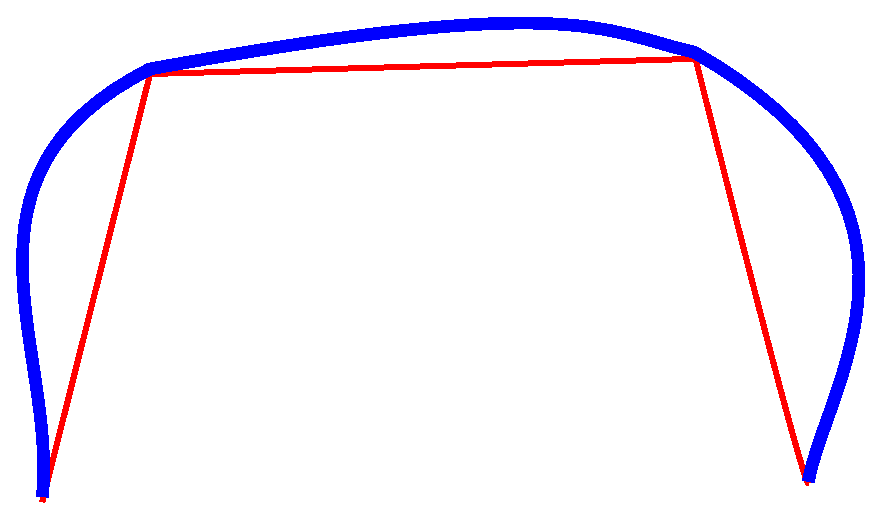
\includegraphics[width=0.6\textwidth]{images/LineGeneralization.eps}
  \caption[A simple example of line generalization.]{\label{figure:LineGeneralization}A simple example of line generalization, where a curve (blue) is represented by a working segment represented by 4 points along the curve connected by three line segments (red). Adding more points increases the accuracy of the generalization.}
\end{figure}


The steps to compressing the a terrain as a drill representation are as follows:

\begin{enumerate}
  \item Compress each segment of the drainage network using Freeman Chain Coding or line generalization.
  \item Encode each drill as an initial pixel and a drill shape.
  \item Compress the drill encoding.
  \item (Optional) Apply further compression techniques, such as 7Zip.
\end{enumerate}

As discussed in Section \ref{section:FamiliesOfFunctions}, a single drill can be encoded per segment of the channel network without significant loss of accuracy. In lieu of this, the various segments of the drainage network can be compressed using a scheme such as Freeman Chain Coding \cite{Freeman:1974:CPL:356625.356627} or line generalization \cite{Ramar72:Polygonalapproximation}. 

Freeman Chain Coding is a lossless method of compressing a line segment in an 8-directional system by storing the initial pixel location and then a chain of movement directions. The simplicity of the representation allows for additional compression, since each subsequent direction can be stored in 3 bits. In addition, taking advantage of the tendency for flows to travel in the same direction for long distances allows each segment to be compressed further by simple run length encoding, or more complex lossless compression.
 
Alternatively, line generalization is a lossy method of compressing a line segment by creating a current guess for the line, called the \textit{working segment}, initialized with the first and last pixel of the line.
% starting with the beginning and ending pixel of a segment and drawing a line between them. 
% This is the initial guess for the line segment. 
The furthest pixel from the working segment, using the 2-norm distance in pixel space, is then added to it, and a new guess is created with all the pixels in the working segment. This process is repeated until the desired accuracy or compression ratio is achieved. An example of this process can be seen in Figure \ref{figure:LineGeneralization}.

Since each line segment of the drainage network is now indexed in the encoding by its starting pixel, each drill can be stored in order of the index of the corresponding segment, and so only needs to be encoded as the shape. The drill encoding then becomes a $2 \times n$ matrix, where $n$ is the number of drills, and can be compressed with any lossless matrix compression scheme that is convenient. 

What is important to note is that Freeman Chain Coding is lossless, so if it is used along with a lossless compression of the drill matrix, the only accuracy lost by this scheme is found in the actual representation itself. To a degree, this is unnecessary since most terrain data is inherently inaccurate to begin with. However, by making the accuracy of the compression (either using lossless, or bounded with line generalization) adjustable, there is an additional level of control put in the hands of the user.

Once the compressed files are written, then can be compressed further with file archive problems such as 7Zip \cite{7z-Pavlov} and gzip. Both provide additional compression with minimal data loss.

\subsection{Results and Discussion of Compression Testing}

The six datasets shown in Figure \ref{figure:SixDatasets} were compressed using the scheme presented in Section \ref{section:CompressionScheme}, as well as image compression techniques PNG and JPEG, and archiving technique 7Zip.
For these tests, the drill was compressed by converting the ASCII data into binary data and storing the Freeman Chain Codes as an optimal series of 3-bit sequences.
The PNG and JPEG files were created using the respective MATLAB implementations, and the 7Zip files were created using the default Ubuntu 11.04 compression option. For the JPEG compression, the chosen bit-depth was 12 bits (because 8 was not enough to store the full range of elevations in the data).

The results of these compressions are presented in Table \ref{table:CompressionResults}.

\begin{table}[t]
  \centering
    \begin{tabular}{| l | l | l | l | l | l | l |}
      \hline
      & Original (Binary) & Original (ASCII) & Drill* & 7Zip & PNG & JPEG \\
      \hline
      HILL1 & 320.0 & 781.3 & 83.7 & 70.4 & 89.0 & 13.7 \\
      \hline
      HILL2 & 320.0 & 781.3 & 161.8 & 101.6 & 138.6 & 20.8 \\
      \hline
      HILL3 & 320.0 & 781.3 & 44.8 & 48.7 & 57.7 & 9.3 \\
      \hline
      MTN1 & 320.0 & 625.4 & 230.4 & 115.7 & 182.4 & 39.9 \\
      \hline
      MTN2 & 320.0 & 651.1 & 8.4 & 130.5 & 145.7 & 36.0 \\
      \hline
      MTN3 & 320.0 & 625.3 & 148.5 & 116.0 & 158.6 & 39.9 \\
      \hline
    \end{tabular}
  \caption[Results for compression scheme tests.]{\label{table:CompressionResults} The resulting files sizes (in KB) of files generated using the Drill, 7Zip, JPEG, and PNG compression schemes for each of the six datasets in Figure \ref{figure:SixDatasets}. Each file's original size is given, as well, for both binary and ASCII representations.}
\end{table}

The drill representation used for each dataset was chosen to be the smallest set of operators whose RMSE was below 5\%. The RMSE of each of the other representations was each 0\% (7Zip and PNG, which are lossless) or near 0\% (JPEG). For the drill representation, an additional compression step was applied, using the archive format 7Zip. The additional compression it provided was small, usually only one or two KBs.

The JPEG compression algorithm is very good. With minimal data loss (on a pixel-by-pixel elevation basis), JPEG outperformed all other compression schemes with regard to compression ratio. However, allowing for a 5\% RMSE, the drill compression is able to significantly outperform JPEG and all other schemes on the MTN2 dataset. As presented in Section \ref{section:FamiliesOfFunctions}, the drill is able to very tightly fit the MTN2 dataset, even with very few pixels included in the channel network. This allows for a very small representation to be compressed. 
If the set of operators that provided the smallest error is used, the MTN2 file size grows to \fbox{CHECK THIS FIGURE} 40.0 KB. This is still comparable to the JPEG scheme, and stores more information than JPEG while introducing very little error. 

The PNG scheme performs well for well-structured data with lots of flat areas (HILL1 and HILL3), due to the run-length nature of the scheme. 7Zip performs well for similar reasons, which is why it does not greatly benefit the drill scheme to use it as an additional step since the originally compressed file is very densely packed. 

Like many compression schemes, the drill is dependent upon the structure of the underlying data, most notably the extracted channel network. Improvements in the generalization of the channel network will improve compression ratios while continuing to limit error. As the results for MTN2 prove, it is possible for the drill to accurately and compactly represent a terrain dataset, and the compression scheme introduced in Section \ref{section:TerrainCompression} is feasible. 
% However, improvements to the drill fitting need to be made, whether they be better functions or a generalization of the extracted channel network, before the compression can be widely used for many datasets.
To make the scheme a practical reality, further development of drill fitting techniques is necessary, as well as a method for pruning and generalizing the channel network. Pruning can be accomplished by applying the Junction Point Balance scheme, discussed later in this thesis in Section \ref{section:JunctionBalance}.


% \section{Machining the Terrain}
% 
% \fbox{Chapter about machining}
% 
% 
% \section{Post-Processing the Terrain}
% 
% \fbox{Chapter about post-processing}


\section{Summary of the Drill Operator}
\label{section:FutureWorkDrillOperator}

Chapter \ref{chapter:DrillOperator} introduced the drill, a mathematical operator that can, with proper placement and shape fitting, represent a terrain dataset with little error (Section \ref{section:DrillAccuracyTests}). 
The drill operator mimics digging out the surface with a circular drill, and as such encodes more information than a simple height field or TIN representation. In addition to its ties to a physical process, the operator also allows for discontinuities to be encoded along the edges of the drill itself. This allows for the representation of cliff faces, such as along channel edges, something height fields and TINs are incapable of. Finally, when storing the drill location as a string of pixels (a channel segment), as discussed in Section \ref{section:FamiliesOfFunctions}, local minima on the surface are prevented.

Three families of drill shapes were tested to determine which represent the surface most accurately. The most accurate drill shape for most terrain datasets is the linear shape, with decreasing accuracy as the degree of the polynomial drill shape increases. Terrain with a higher level of detail around its extracted channels (i.e. mountainous terrain) is more suited for drill representations, but all terrains tested were adequately represented.

In addition, the drill operator was shown to be an effective mechanism for compressing terrain data, by storing the compressed channel network along with the encoded set of drill operators that represent the surface. The drill representation does not compress better than JPEG with regard to its compression ratio, but it stores more information and does not smooth the surface. Further improvements to the operator and the extraction of the channel network will greatly improve this compression scheme.

With a representation that can represent legal terrains, the capacity for more accurate data collection exists. This representation is still limited by its reliance on surface sampled elevation collection, as errors in the data are impossible to avoid. As terrain representations that can model more complex terrain formations compactly and robustly are developed, data collection techniques will be developed to take advantage of them. The drill operator is a step in that direction.

\section{Future Work for the Drill Operator}

There are several extensions to be made to the drill terrain representation. The first is the method in which the drill is fit to the surface can be extended in a variety of ways. Each channel segment of the terrain should not only have its own drill parameters, but its own drill shape altogether. In some areas, a linear drill is better suited to be fit to the terrain, whereas in others a quadratic would work better. Along those same lines, more drill shapes will be incorporated into the framework, including ones that do not follow the definition of a function (allowing for spherical drills for caves and overhangs). 

Does the order of the application of the drills matter? We can mimic the process of ``machining'' the terrain by applying broader drills first, and then refining the individual channels with finer and finer drills, like one would machine a piece of metal. Along similar lines, there are various post-processing techniques that can be applied to a regenerated terrain. For instance, the ODETLAP algorithm can smooth out outlier pixels while simultaneously filling in gaps. This would allow the use of fewer, more precise drills along the channel network without worrying about touching all parts of the terrain. However, ODETLAP can overly-smooth the surface, eliminating discontinuities. To minimize this issue, the drills can be re-applied to the terrain after the ODETLAP procedure.

In order to extend the drill operator, a method will be developed to quickly and accurately identify the optimal parameters for the drill fitting. As it stands, to find the representation with the minimum error, a brute force method was used. However, this can certainly be optimized. This thesis did not focus on temporal optimization of the algorithms, but this needs to be a focus moving forward in order to truly make the drill representation practical for data collection and compression.

% There are several ways in which the drill-fitting algorithm can be optimized. 
% The first is by storing channel segments as opposed to individual pixels, such as with Freeman chain codes \cite{Freeman:1974:CPL:356625.356627} or line generalization \cite{Ramar72:Polygonalapproximation}. If a channel network can be stored as a series of segments, with begin points, end points, and channel trajectories, along with a function of drill shape (allowing it to change along the length of the channel), then the overall storage of a terrain can be greatly reduced. Storing the channels as trajectories also allows for a post-processing step that forces the trajectories to be monotonic and decreasing, thus forcing a lack of local minima and allowing the drill operator to adhere to the second criterion for a ``legal terrain'' described in Section \ref{section:intro}.
% With regards to temporal optimization, the drill creation algorithm bottlenecks at the function fitting. A better method of function fitting may significantly improve the performance of the algorithm. Drills can be any shape, including simple cones, and have a width along the bottom. If the restriction that the drill shape functions be monotonic and increasing is lifted, a drill can be ball-shaped, which could model caves. These new parameters would allow for more customizability while maintaining a small memory footprint.

Two more operators will be added to the set of operators: the erosion operator, and the mudslide operator. The erosion operator picks up sediment from a high elevation and deposits it at a lower elevation, and the mudslide operator adds sediment to the terrain along a trajectory. Deeper mathematics of these three operators will be explored, including how to define the composition of two operations, and whether that creates a group over the composition operation.  
% In addition, 

We will investigate ways to post-process terrain to deal with small areas untouched by drill operations. A simple interpolation of the untouched areas may be a solution, or more sophisticated algorithms may be more useful. Also, the system, as it currently stands, has three user-defined parameters ($\tau$, $w$, and $k$). We will investigate ways to automatically determine the ideal value for each of these parameters before operation extraction, thus not relying on user knowledge to create the best representation. Ideally, every operator will store its own value for $k$.

Finally, terrain DEM data is isometric to greyscale image data. To date there has been a great deal of work done in applying algorithms for images to terrain, especially in the area of terrain compression. However, measuring error (or dissimilarity) using the plethora of image dissimilarity measures has not been explored to its fullest. In the future, the representations presented in this thesis will use more sophisticated image dissimilarity measures (such as a more direct application of the Earth Mover's Distance \cite{Rubner:2000:EMD:365875.365881}).